%        File: arfc-beamer.tex
%     Created: Sun May 5 10:00 PM 2013 C
%


%\documentclass[11pt,handout]{beamer}
\documentclass[9pt]{beamer}
\usetheme[white]{Illinois}
\title[Short Title]{Fluoride-Salt-Cooled High-Temperature Reactor Generative Design Optimization with Evolutionary Algorithms}
\subtitle[short subtitle]{Ph.D. Final Defense}
\author[Your Name]{Gwendolyn J.Y. Chee}
\date[09.13.2021]{August 12, 2022}
\institute{
Dept. of Nuclear, Plasma and Radiological Engineering \\ University of Illinois at Urbana-Champaign
}

%\usepackage{bbding}
\usepackage{amsfonts}
\usepackage{amsmath}
\usepackage{xspace}
\usepackage{graphicx}
\usepackage{booktabs} % nice rules for tables
\usepackage{microtype} % if using PDF
\usepackage{bigints}
\usepackage{minted}

\newcommand{\Cyclus}{\textsc{Cyclus}\xspace}%
\newcommand{\Cycamore}{\textsc{Cycamore}\xspace}%
\newcommand{\deploy}{\texttt{d3ploy}\xspace}%
\newcommand{\units}[1] {\:\text{#1}}%
\newcommand{\SN}{S$_N$}%{S$_\text{N}$}%{$S_N$}%
\DeclareMathOperator{\erf}{erf}
%I need some complimentary error funcitons... 
\DeclareMathOperator{\erfc}{erfc}
%page numbers
\setbeamertemplate{footline}[page number]
\setbeamertemplate{caption}[numbered]
%Those icons in the references are terrible looking
\setbeamertemplate{bibliography item}[text]

\usepackage{tkz-euclide}
\usepackage{tikz}
\usetikzlibrary{positioning, arrows, decorations, shapes}

\usetikzlibrary{shapes.geometric,arrows}
\tikzstyle{process} = [rectangle, rounded corners, minimum width=3cm, minimum height=1cm,text centered, draw=black, fill=blue!30]
\tikzstyle{object} = [ellipse, rounded corners, minimum width=3cm, minimum height=1cm,text centered, draw=black, fill=green!30]
\tikzstyle{arrow} = [thick,->,>=stealth]

\definecolor{illiniblue}{HTML}{B1C6E2}
\definecolor{illiniorange}{HTML}{f8c2a2}
\definecolor{illinigreen}{HTML}{a0deb1}
\definecolor{grey}{HTML}{dce3de}
\usetikzlibrary{shapes.geometric, arrows}
\tikzstyle{oblock} = [rectangle, draw, fill=illiniorange, 
text width=9em, text centered, rounded corners, minimum height=4em]
\tikzstyle{bblock} = [rectangle, draw, fill=illiniblue, 
text width=8em, text centered, rounded corners, minimum height=4em]
\tikzstyle{gblock} = [rectangle, draw, fill=illinigreen, 
text width=8em, text centered, rounded corners, minimum height=4em]
\tikzstyle{lgblock} = [rectangle, draw, fill=illinigreen, 
text width=9em, text centered, rounded corners, minimum height=4em]
\tikzstyle{noblock} = [rectangle,
text width=8em, text centered, minimum height=4em]
\tikzstyle{greyblock} = [rectangle, fill=grey, 
text width=8em, minimum height=4em, rounded corners]
\tikzstyle{lgreyblock} = [rectangle, fill=grey, 
text width=9em, minimum height=4em, rounded corners]
\tikzstyle{llgreyblock} = [rectangle, fill=grey, 
text width=20em, minimum height=4em, rounded corners]
\tikzstyle{arrow} = [thick,->,>=stealth]

\definecolor{fhrblue}{HTML}{0000ff}
\definecolor{fhrgrey}{HTML}{808080}
\definecolor{fhrred}{HTML}{f10a0a}
\definecolor{fhrgreen}{HTML}{2f6d39}
\definecolor{fhryellow}{HTML}{fdfe36}

\usepackage{tabularx}
\newcolumntype{b}{>{\hsize=1.0\hsize}X}
\newcolumntype{s}{>{\hsize=.5\hsize}X}
\newcolumntype{m}{>{\hsize=.75\hsize}X}
\newcolumntype{x}{>{\hsize=.25\hsize}X}
\newcolumntype{L}{>{\raggedright\arraybackslash}X}
\newcolumntype{R}{>{\raggedleft\arraybackslash}X}
\def\arraystretch{1}
%%%% Acronym support
\usepackage{multirow}
\usepackage{graphicx}
\usepackage{subcaption}
\usepackage{booktabs}% http://ctan.org/pkg/booktabs
\newcommand{\tabitem}{~~\llap{\textbullet}~~}
\usepackage[acronym,toc]{glossaries}
%\newacronym{<++>}{<++>}{<++>}
\newacronym[longplural={metric tons of heavy metal}]{MTHM}{MTHM}{metric ton of heavy metal}
\newacronym{3D CAD}{3D CAD}{three-dimensional Computer-Aided Design}
\newacronym{AHTR}{AHTR}{Advanced High Temperature Reactor}
\newacronym{AI}{AI}{artificial intelligence}
\newacronym{AMAFT}{AMAFT}{Additive Manufacturing as an Alternative Fabrication Technique}
\newacronym{ANDRA}{ANDRA}{Agence Nationale pour la gestion des D\'echets RAdioactifs, the French National Agency for Radioactive Waste Management}
\newacronym{ANL}{ANL}{Argonne National Laboratory}
\newacronym{ANS}{ANS}{American Nuclear Society}
\newacronym{API}{API}{application programming interface}
\newacronym{ARE}{ARE}{Aircraft Reactor Experiment}
\newacronym{ARFC}{ARFC}{Advanced Reactors and Fuel Cycles}
\newacronym{BP}{BP}{burnable poison}
\newacronym{CFD}{CFD}{Computational Fluid Dynamics}
\newacronym{CEA}{CEA}{Commissariat \`a l'\'Energie Atomique et aux \'Energies Alternatives}
\newacronym{CI}{CI}{continuous integration}
\newacronym{CIEMAT}{CIEMAT}{Centro de Investigaciones Energéticas, Medioambientales y Tecnológicas}
\newacronym{CNEN}{CNEN}{Comiss\~{a}o Nacional de Energia Nuclear}
\newacronym{CNERG}{CNERG}{Computational Nuclear Engineering Research Group}
\newacronym{CNRS}{CNRS}{Le Centre National De La Recherche Scientifique}
\newacronym{COSI}{COSI}{Commelini-Sicard}
\newacronym{COTS}{COTS}{commercial, off-the-shelf}
\newacronym{CR}{CR}{control rod}
\newacronym{CSNF}{CSNF}{commercial spent nuclear fuel}
\newacronym{CTAH}{CTAHs}{Coiled Tube Air Heaters}
\newacronym{CUBIT}{CUBIT}{CUBIT Geometry and Mesh Generation Toolkit}
\newacronym{CURIE}{CURIE}{Centralized Used Fuel Resource for Information Exchange}
\newacronym{CVI}{CVI}{chemical vapor infiltration}
\newacronym{CZP}{CZP}{cold zero power}
\newacronym{DEAP}{DEAP}{Distributed Evolutionary Algorithms in Python}
\newacronym{DESAE}{DESAE}{Dynamic Analysis of Nuclear Energy Systems Strategies}
\newacronym{DNBR}{DNBR}{Departure from nucleate boiling ratio}
\newacronym{DNP}{DNP}{delayed neutron precursor}
\newacronym{DOE}{DOE}{Department of Energy}
\newacronym{dpa}{dpa}{displacements per atom}
\newacronym{DRACS}{DRACS}{Direct Reactor Auxiliary Cooling System}
\newacronym{DRE}{DRE}{dynamic resource exchange}
\newacronym{DSNF}{DSNF}{DOE spent nuclear fuel}
\newacronym{DYMOND}{DYMOND}{Dynamic Model of Nuclear Development }
\newacronym{EA}{EA}{evolutionary algorithm}
\newacronym{EBM}{EBM}{electron beam melting}
\newacronym{EBS}{EBS}{Engineered Barrier System}
\newacronym{EDF}{EDF}{Électricité de France}
\newacronym{EDZ}{EDZ}{Excavation Disturbed Zone}
\newacronym{EG}{EG}{Evaluation Group}
\newacronym{EIA}{EIA}{U.S. Energy Information Administration}
\newacronym{EPA}{EPA}{Environmental Protection Agency}
\newacronym{EPR}{EPR}{European Pressurized Reactors}
\newacronym{EPRI}{EPRI}{Electric Power Research Institute}
\newacronym{EP}{EP}{Engineering Physics}
\newacronym{EU}{EU}{European Union}
\newacronym{FCM}{FCM}{fully ceramic microencapsulated}
\newacronym{FCO}{FCO}{Fuel Cycle Options}
\newacronym{FCT}{FCT}{Fuel Cycle Technology}
\newacronym{FD}{FD}{fission density}
\newacronym{FEHM}{FEHM}{Finite Element Heat and Mass Transfer}
\newacronym{FEPs}{FEPs}{Features, Events, and Processes}
\newacronym{FHR}{FHR}{Fluoride-Salt-Cooled High-Temperature Reactor}
\newacronym{FLiBe}{FLiBe}{Fluoride-Lithium-Beryllium}
\newacronym{FM}{FM}{ferritic/martensitic}
\newacronym{FP}{FP}{Fission Product}
\newacronym{GA}{GA}{genetic algorithm}
\newacronym{GDSE}{GDSE}{Generic Disposal System Environment}
\newacronym{GDSM}{GDSM}{Generic Disposal System Model}
\newacronym{Georgia Tech}{Georgia Tech}{Georgia Institute of Technology}
\newacronym{GENIUSv1}{GENIUSv1}{Global Evaluation of Nuclear Infrastructure Utilization Scenarios, Version 1}
\newacronym{GENIUSv2}{GENIUSv2}{Global Evaluation of Nuclear Infrastructure Utilization Scenarios, Version 2}
\newacronym{GENIUS}{GENIUS}{Global Evaluation of Nuclear Infrastructure Utilization Scenarios}
\newacronym{GFR}{GFR}{Gas-Cooled Fast Reactor}
\newacronym{GHG}{GHG}{Greenhouse Gas}
\newacronym{GUI}{GUI}{graphical user interface}
\newacronym{HEM}{HEM}{Homogenous Equilibrium Mixture}
\newacronym{HFIR}{HFIR}{High Flux Isotope Reactor}
\newacronym{HLW}{HLW}{high level waste}
\newacronym{HM}{HM}{heavy metal}
\newacronym{HPC}{HPC}{high-performance computing}
\newacronym{HTC}{HTC}{high-throughput computing}
\newacronym{HTGR}{HTGR}{High Temperature Gas-Cooled Reactor}
\newacronym{HZP}{HZP}{hot zero power}
\newacronym{IAEA}{IAEA}{International Atomic Energy Agency}
\newacronym{IEMA}{IEMA}{Illinois Emergency Mangament Agency}
\newacronym{IHLRWM}{IHLRWM}{International High Level Radioactive Waste Management}
\newacronym{INL}{INL}{Idaho National Laboratory}
\newacronym{IPRR1}{IRP-R1}{Instituto de Pesquisas Radioativas Reator 1}
\newacronym{IRP}{IRP}{Integrated Research Project}
\newacronym{IRSN}{IRSN}{Institute for Radiological Protection and Nuclear Safety}
\newacronym{ISFSI}{ISFSI}{Independent Spent Fuel Storage Installation}
\newacronym{ISRG}{ISRG}{Independent Student Research Group}
\newacronym{JAEA}{JAEA}{Japanese Atomic Energy Agency}
\newacronym{JFNK}{JFNK}{Jacobian-Free Newton Krylov}
\newacronym{LANL}{LANL}{Los Alamos National Laboratory}
\newacronym{LBNL}{LBNL}{Lawrence Berkeley National Laboratory}
\newacronym{LCOE}{LCOE}{levelized cost of electricity}
\newacronym{L-DED}{L-DED}{laser directed energy deposition}
\newacronym{LDRD}{LDRD}{laboratory directed research and development}
\newacronym{LEU}{LEU}{low-enriched uranium}
\newacronym{LFR}{LFR}{Lead-Cooled Fast Reactor}
\newacronym{LLNL}{LLNL}{Lawrence Livermore National Laboratory}
\newacronym{LMFBR}{LMFBR}{Liquid Metal Fast Breeder Reactor}
\newacronym{LOFC}{LOFC}{Loss of Forced Cooling}
\newacronym{LOHS}{LOHS}{Loss of Heat Sink}
\newacronym{LOLA}{LOLA}{Loss of Large Area}
\newacronym{LP}{LP}{linear program}
\newacronym{LPD}{LPD}{Local power density}
\newacronym{LWR}{LWR}{Light Water Reactor}
\newacronym{MA}{MA}{minor actinide}
\newacronym{MCNP}{MCNP}{Monte Carlo N-Particle code}
\newacronym{MHC}{MHC}{molybdenum–hafnium carbide alloy}
\newacronym{MILP}{MILP}{mixed-integer linear program}
\newacronym{MIT}{MIT}{Massachusetts Institute of Technology}
\newacronym{MOAB}{MOAB}{Mesh-Oriented datABase}
\newacronym{MOOSE}{MOOSE}{Multiphysics Object-Oriented Simulation Environment}
\newacronym{MOSART}{MOSART}{Molten Salt Actinide Recycler and Transmuter}
\newacronym{MOX}{MOX}{mixed oxide}
\newacronym{MPI}{MPI}{Message Passing Interface}
\newacronym{MSBR}{MSBR}{Molten Salt Breeder Reactor}
\newacronym{MSFR}{MSFR}{Molten Salt Fast Reactor}
\newacronym{MSRE}{MSRE}{Molten Salt Reactor Experiment}
\newacronym{MSR}{MSR}{Molten Salt Reactor}
\newacronym{NAGRA}{NAGRA}{National Cooperative for the Disposal of Radioactive Waste}
\newacronym{NEA}{NEA}{Nuclear Energy Agency}
\newacronym{NEM}{NEM}{Nodal Expansion Method}
\newacronym{NEAMS}{NEAMS}{Nuclear Engineering Advanced Modeling and Simulation}
\newacronym{NESTLE}{NESTLE}{Nodal Eigenvalue, Steady-state, Transient, Le core Evaluator}
\newacronym{NEUP}{NEUP}{Nuclear Energy University Programs}
\newacronym{NFC}{NFC}{Nuclear Fuel Cycle}
\newacronym{NFCSim}{NFCSim}{Nuclear Fuel Cycle Simulator}
\newacronym{NGNP}{NGNP}{Next Generation Nuclear Plant}
\newacronym{NMR-50}{NMR-50}{Purdue Novel Modular Reactor}
\newacronym{NMWPC}{NMWPC}{Nuclear MW Per Capita}
\newacronym{NNL}{NNL}{National Nuclear Laboratory}
\newacronym{NNSA}{NNSA}{National Nuclear Security Administration}
\newacronym{NPRE}{NPRE}{Department of Nuclear, Plasma, and Radiological Engineering}
\newacronym{NQA1}{NQA-1}{Nuclear Quality Assurance - 1}
\newacronym{NRC}{NRC}{Nuclear Regulatory Commission}
\newacronym{NSF}{NSF}{National Science Foundation}
\newacronym{NSGA-II}{NSGA-II}{Non-dominated Sorting Genetic Algorithm II}
\newacronym{NSSC}{NSSC}{Nuclear Science and Security Consortium}
\newacronym{NUWASTE}{NUWASTE}{Nuclear Waste Assessment System for Technical Evaluation}
\newacronym{NWF}{NWF}{Nuclear Waste Fund}
\newacronym{NWTRB}{NWTRB}{Nuclear Waste Technical Review Board}
\newacronym{OCRWM}{OCRWM}{Office of Civilian Radioactive Waste Management}
\newacronym{OECD}{OECD}{Organisation for Economic Co-operation and Development}
\newacronym{ORION}{ORION}{ORION}
\newacronym{ORNL}{ORNL}{Oak Ridge National Laboratory}
\newacronym{PARCS}{PARCS}{Purdue Advanced Reactor Core Simulator}
\newacronym{PCA}{PCA}{Particle Collision Algorithm}
\newacronym{PBAHTR}{PB-AHTR}{Pebble Bed Advanced High Temperature Reactor}
\newacronym{PBFHR}{PB-FHR}{Pebble-Bed Fluoride-Salt-Cooled High-Temperature Reactor}
\newacronym{PDE}{PDE}{Partial Differential Equation}
\newacronym{PEI}{PEI}{Peak Environmental Impact}
\newacronym{PH}{PRONGHORN}{PRONGHORN}
\newacronym{PIRT}{PIRT}{Phenomena Identification and Ranking Table}
\newacronym{PPF}{PPF}{Power peaking factor}
\newacronym{PRIS}{PRIS}{Power Reactor Information System}
\newacronym{PRKE}{PRKE}{Point Reactor Kinetics Equations}
\newacronym{PSPG}{PSPG}{Pressure-Stabilizing/Petrov-Galerkin}
\newacronym{PWAR}{PWAR}{Pratt and Whitney Aircraft Reactor}
\newacronym{PWR}{PWR}{Pressurized Water Reactor}
\newacronym{PyNE}{PyNE}{Python toolkit for Nuclear Engineering}
\newacronym{PyRK}{PyRK}{Python for Reactor Kinetics}
\newacronym{PyPI}{PyPI}{The Python Package Index}
\newacronym{QA}{QA}{quality assurance}
\newacronym{RDD}{RD\&D}{Research Development and Demonstration}
\newacronym{RD}{R\&D}{Research and Development}
\newacronym{REALM}{REALM}{Reactor Evolutionary Algorithm Optimizer}
\newacronym{REE}{REE}{rare earth element}
\newacronym{RELAP}{RELAP}{Reactor Excursion and Leak Analysis Program}
\newacronym{RIA}{RIA}{Reactivity Insertion Accident}
\newacronym{RIF}{RIF}{Region-Institution-Facility}
\newacronym{ROLLO}{ROLLO}{Reactor evOLutionary aLgorithm Optimizer}
\newacronym{SA}{SA}{Simulation Annealing}
\newacronym{SCK CEN}{SCK CEN}{Studiecentrum voor Kernenergie}
\newacronym{SCWR}{SCWR}{Supercritical-Water-Cooled Reactor}
\newacronym{SFR}{SFR}{Sodium-Cooled Fast Reactor}
\newacronym{SF-TMSR}{SF-TMSR}{Solid Fuel Thorium Molten Salt Reactor}
\newacronym{SiC}{SiC}{silicon carbide}
\newacronym{SINAP}{SINAP}{Shanghai Institute of Applied Physics}
\newacronym{SINDAG}{SINDA{\textbackslash}G}{Systems Improved Numerical Differencing Analyzer $\backslash$ Gaski}
\newacronym{SKB}{SKB}{Svensk K\"{a}rnbr\"{a}nslehantering AB}
\newacronym{SLM}{SLM}{selective laser melting}
\newacronym{SmAHTR}{SmAHTR}{Small Modular AHTR}
\newacronym{SNF}{SNF}{spent nuclear fuel}
\newacronym{SNL}{SNL}{Sandia National Laboratory}
\newacronym{SLM}{SLM}{selective laser melting}
\newacronym{STC}{STC}{specific temperature change}
\newacronym{SUPG}{SUPG}{Streamline-Upwind/Petrov-Galerkin}
\newacronym{SWF}{SWF}{Separations and Waste Forms}
\newacronym{SWU}{SWU}{Separative Work Unit}
\newacronym{TCR}{TCR}{Transformational Challenge Reactor}
\newacronym{TRIGA}{TRIGA}{Training Research Isotope General Atomic}
\newacronym{TRISO}{TRISO}{Tristructural Isotropic}
\newacronym{TSM}{TSM}{Total System Model}
\newacronym{TSPA}{TSPA}{Total System Performance Assessment for the Yucca Mountain License Application}
\newacronym{ThOX}{ThOX}{thorium oxide}
\newacronym{UCB}{UCB}{University of California Berkeley}
\newacronym{UFD}{UFD}{Used Fuel Disposition}
\newacronym{UML}{UML}{Unified Modeling Language}
\newacronym{UOX}{UOX}{uranium oxide}
\newacronym{UQ}{UQ}{uncertainty quantification}
\newacronym{US}{US}{United States}
\newacronym{USC}{USC}{University of South Carolina}
\newacronym{UIUC}{UIUC}{University of Illinois at Urbana-Champaign}
\newacronym{UT Austin}{UT Austin}{The University of Texas at Austin}
\newacronym{VHTR}{VHTR}{Very-High-Temperature Reactor}
\newacronym{VV}{V\&V}{verification and validation}
\newacronym{WCT}{WCT}{wall-clock-time}
\newacronym{YMR}{YMR}{Yucca Mountain Repository Site}

%\makeglossaries
\setbeamerfont{subsection in toc}{size=\scriptsize}

%try to get rid of header on title page\dots
\makeatletter
    \newenvironment{withoutheadline}{
        \setbeamertemplate{headline}[default]
        \def\beamer@entrycode{\vspace*{-\headheight}}
    }{}
\makeatother

% add slide numbers
\makeatother
\setbeamertemplate{footline}
{
  \leavevmode%
  \hbox{%
    \rightline{\insertframenumber{} / \inserttotalframenumber\hspace*{1ex}}
  }%
  \vskip0pt%
}
\makeatletter

\begin{document}
%%%%%%%%%%%%%%%%%%%%%%%%%%%%%%%%%%%%%%%%%%%%%%%%%%%%%%%%%%%%%
%% From uw-beamer Here's a handy bit of code to place at 
%% the beginning of your presentation (after \begin{document}):
\newcommand*{\alphabet}{ABCDEFGHIJKLMNOPQRSTUVWXYZabcdefghijklmnopqrstuvwxyz}
\newlength{\highlightheight}
\newlength{\highlightdepth}
\newlength{\highlightmargin}
\setlength{\highlightmargin}{2pt}
\settoheight{\highlightheight}{\alphabet}
\settodepth{\highlightdepth}{\alphabet}
\addtolength{\highlightheight}{\highlightmargin}
\addtolength{\highlightdepth}{\highlightmargin}
\addtolength{\highlightheight}{\highlightdepth}
\newcommand*{\Highlight}{\rlap{\textcolor{HighlightBackground}{\rule[-\highlightdepth]{\linewidth}{\highlightheight}}}}
%%%%%%%%%%%%%%%%%%%%%%%%%%%%%%%%%%%%%%%%%%%%%%%%%%%%%%%%%%%%%
%%--------------------------------%%
\begin{withoutheadline}
\frame{
  \titlepage
}
\end{withoutheadline}

%%--------------------------------%%
\AtBeginSection[]{
\begin{frame}
  \frametitle{Outline}
  \tableofcontents[currentsection]
\end{frame}
}

\section{Introduction}
\subsection{Overview}
\begin{frame}
    \frametitle{Overview}
    \textbf{Additive manufacturing will radically transform reactor design.}
    \vspace{0.5cm}

    For this dissertation, I successfully
    \begin{enumerate}
        \item Furthered our understanding of the \gls{AHTR} design's complexities 
        through neutronics and thermal-hydraulics modeling
        \item Created an open-source tool that enables nuclear reactor design 
        evolutionary algorithm optimization for non-conventional reactor geometries and fuel 
        distributions
        \item Applied the optimization tool to the \gls{AHTR} design 
    \end{enumerate}

\end{frame}
\subsection{Background: AHTR Model Development}
\begin{frame}
    \frametitle{Why Generation IV Reactors?}
    \begin{itemize}
      \item Energy use and production contribute $\frac{2}{3}$ of Greenhouse Gas 
      emissions \cite{noauthor_climate_2018}
      \item  Large scale emissions-free nuclear power deployment could 
      significantly reduce GHG production but faces both cost and perceived 
      safety challenges 
      \item The Generation IV International Forum identified six systems 
      that promise significant advances in safety, sustainability, efficiency, 
      and cost over existing designs: GFR, LFR, MSR, SFR, SCWR, and VHTR. 
      \begin{figure}[htbp!]
          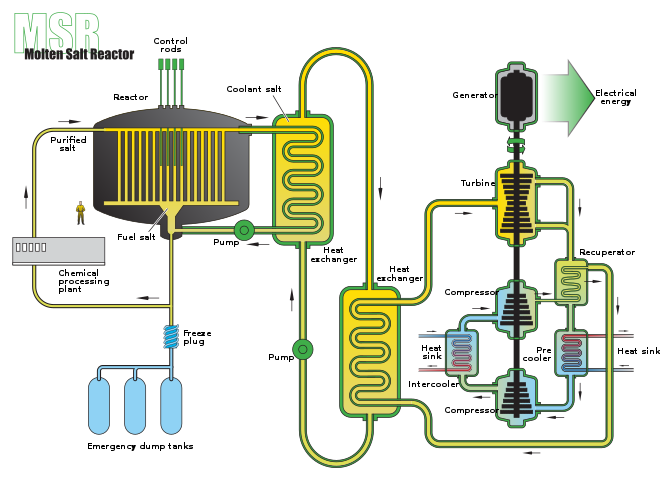
\includegraphics[height=3cm]{figures/msr}
          \hspace{1cm}
          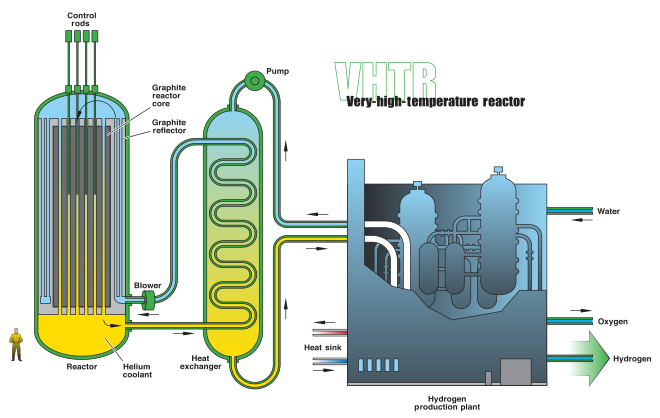
\includegraphics[height=3cm]{figures/vhtr}
          \caption{Left: Molten Salt Reactor System, Right: Very High-Temperature
          Reactor System \cite{gif_technology_2002}. }
      \end{figure}
    \end{itemize}
  \end{frame}
\begin{frame}
  \frametitle{MSRs and VHTRs}
  \begin{block}{Molten Salt Reactor (MSR) System Advantages}
    \begin{itemize}
      \item Molten Fluoride Salts: chemical stability, low vapor pressure at 
      high temperatures, good heat transfer, resistance against radiation damage
      \item Inherent System Safety: passive cooling, fail-safe drainage
    \end{itemize}
  \end{block}
  \vspace{-0.25cm}
  \begin{block}{Very High Temperature Reactor (VHTR) System Advantages}
    \begin{itemize}
      \item TRISO Fuel: withstands high burnup and temperature
      \item High Outlet Temperature: increases power conversion efficiency, reduces 
      waste heat generation, enables high-temperature heat applications 
    \end{itemize}
  \end{block}
  \begin{figure}[htbp!]
    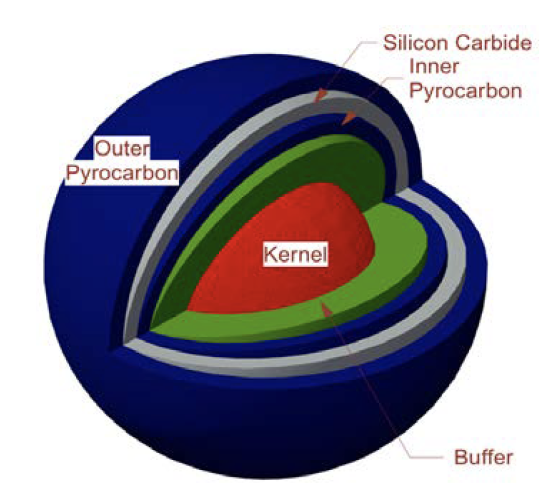
\includegraphics[width=0.2\linewidth]{../docs/figures/ahtr-triso.png}
    \caption{TRISO particle. Diameter: $\sim 8mm$}
\end{figure}
\end{frame}
\begin{frame}
  \frametitle{\acrlong{FHR}}
  FHR concept combines the best aspects of MSR and VHTR:
  low-pressure liquid fluoride-salt coolant and TRISO fuel 
  \begin{block}{\acrfull{FHR} Advantages}
    \begin{itemize}
      \item Molten salt coolant vs. VHTR helium coolant: superior cooling, 
      moderating properties, low operating pressure, large thermal margin
      \item TRISO fuel vs. MSR circulating liquid fuel: solid fuel cladding 
      adds an extra barrier to fission product release
    \end{itemize}
  \end{block}
  \begin{figure}[]
    \centering
    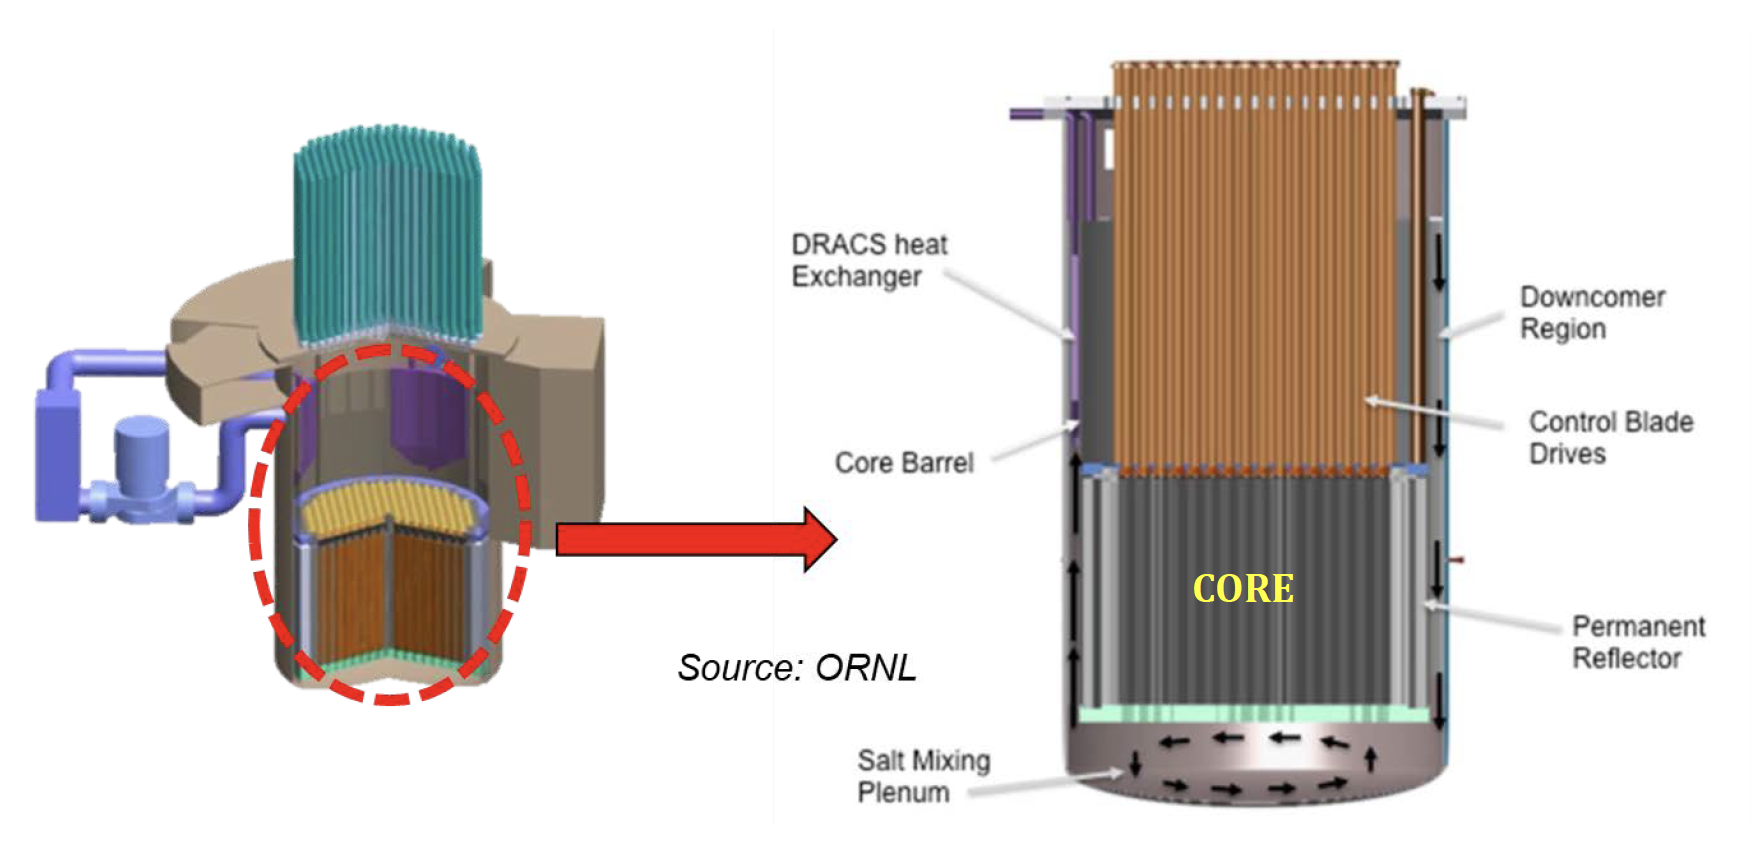
\includegraphics[width=0.5\linewidth]{../docs/figures/reactor-schematic.png} 
    \caption{\acrfull{AHTR} schematic (left) and vessel (right) reproduced from
    \cite{noauthor_fluoride_nodate}.}
\end{figure}
\end{frame}
\begin{frame}
  \frametitle{Advanced High Temperature Reactor Design}
    \begin{itemize}
      \item Design developed by Oak Ridge National Laboratory
      \item Prismatic FHR design with 252 hexagonal fuel assemblies consisting of 
      18 fuel planks arranged in 3 diamond-shaped sectors. 
    \end{itemize}
  \begin{figure}[]
    \centering
    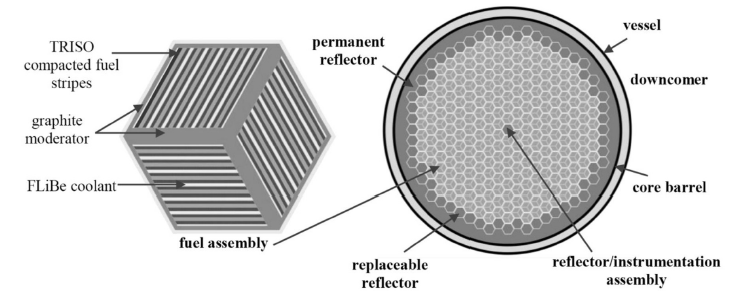
\includegraphics[width=0.9\linewidth]{../docs/figures/ahtr.png} 
    \caption{\acrlong{AHTR} fuel assembly (left) and core configuration (right) 
    reproduced from \cite{ramey_monte_2018}.}
    \label{fig:ahtr}
\end{figure}
\end{frame}

\begin{frame}
  \frametitle{Advanced High Temperature Reactor Geometry}
  The AHTR fuel has a \emph{triple heterogeneity}: hexagonal fuel elements with 
  fuel planks, and TRISO particles embedded in stripes within each plank.
  \begin{figure}[]
    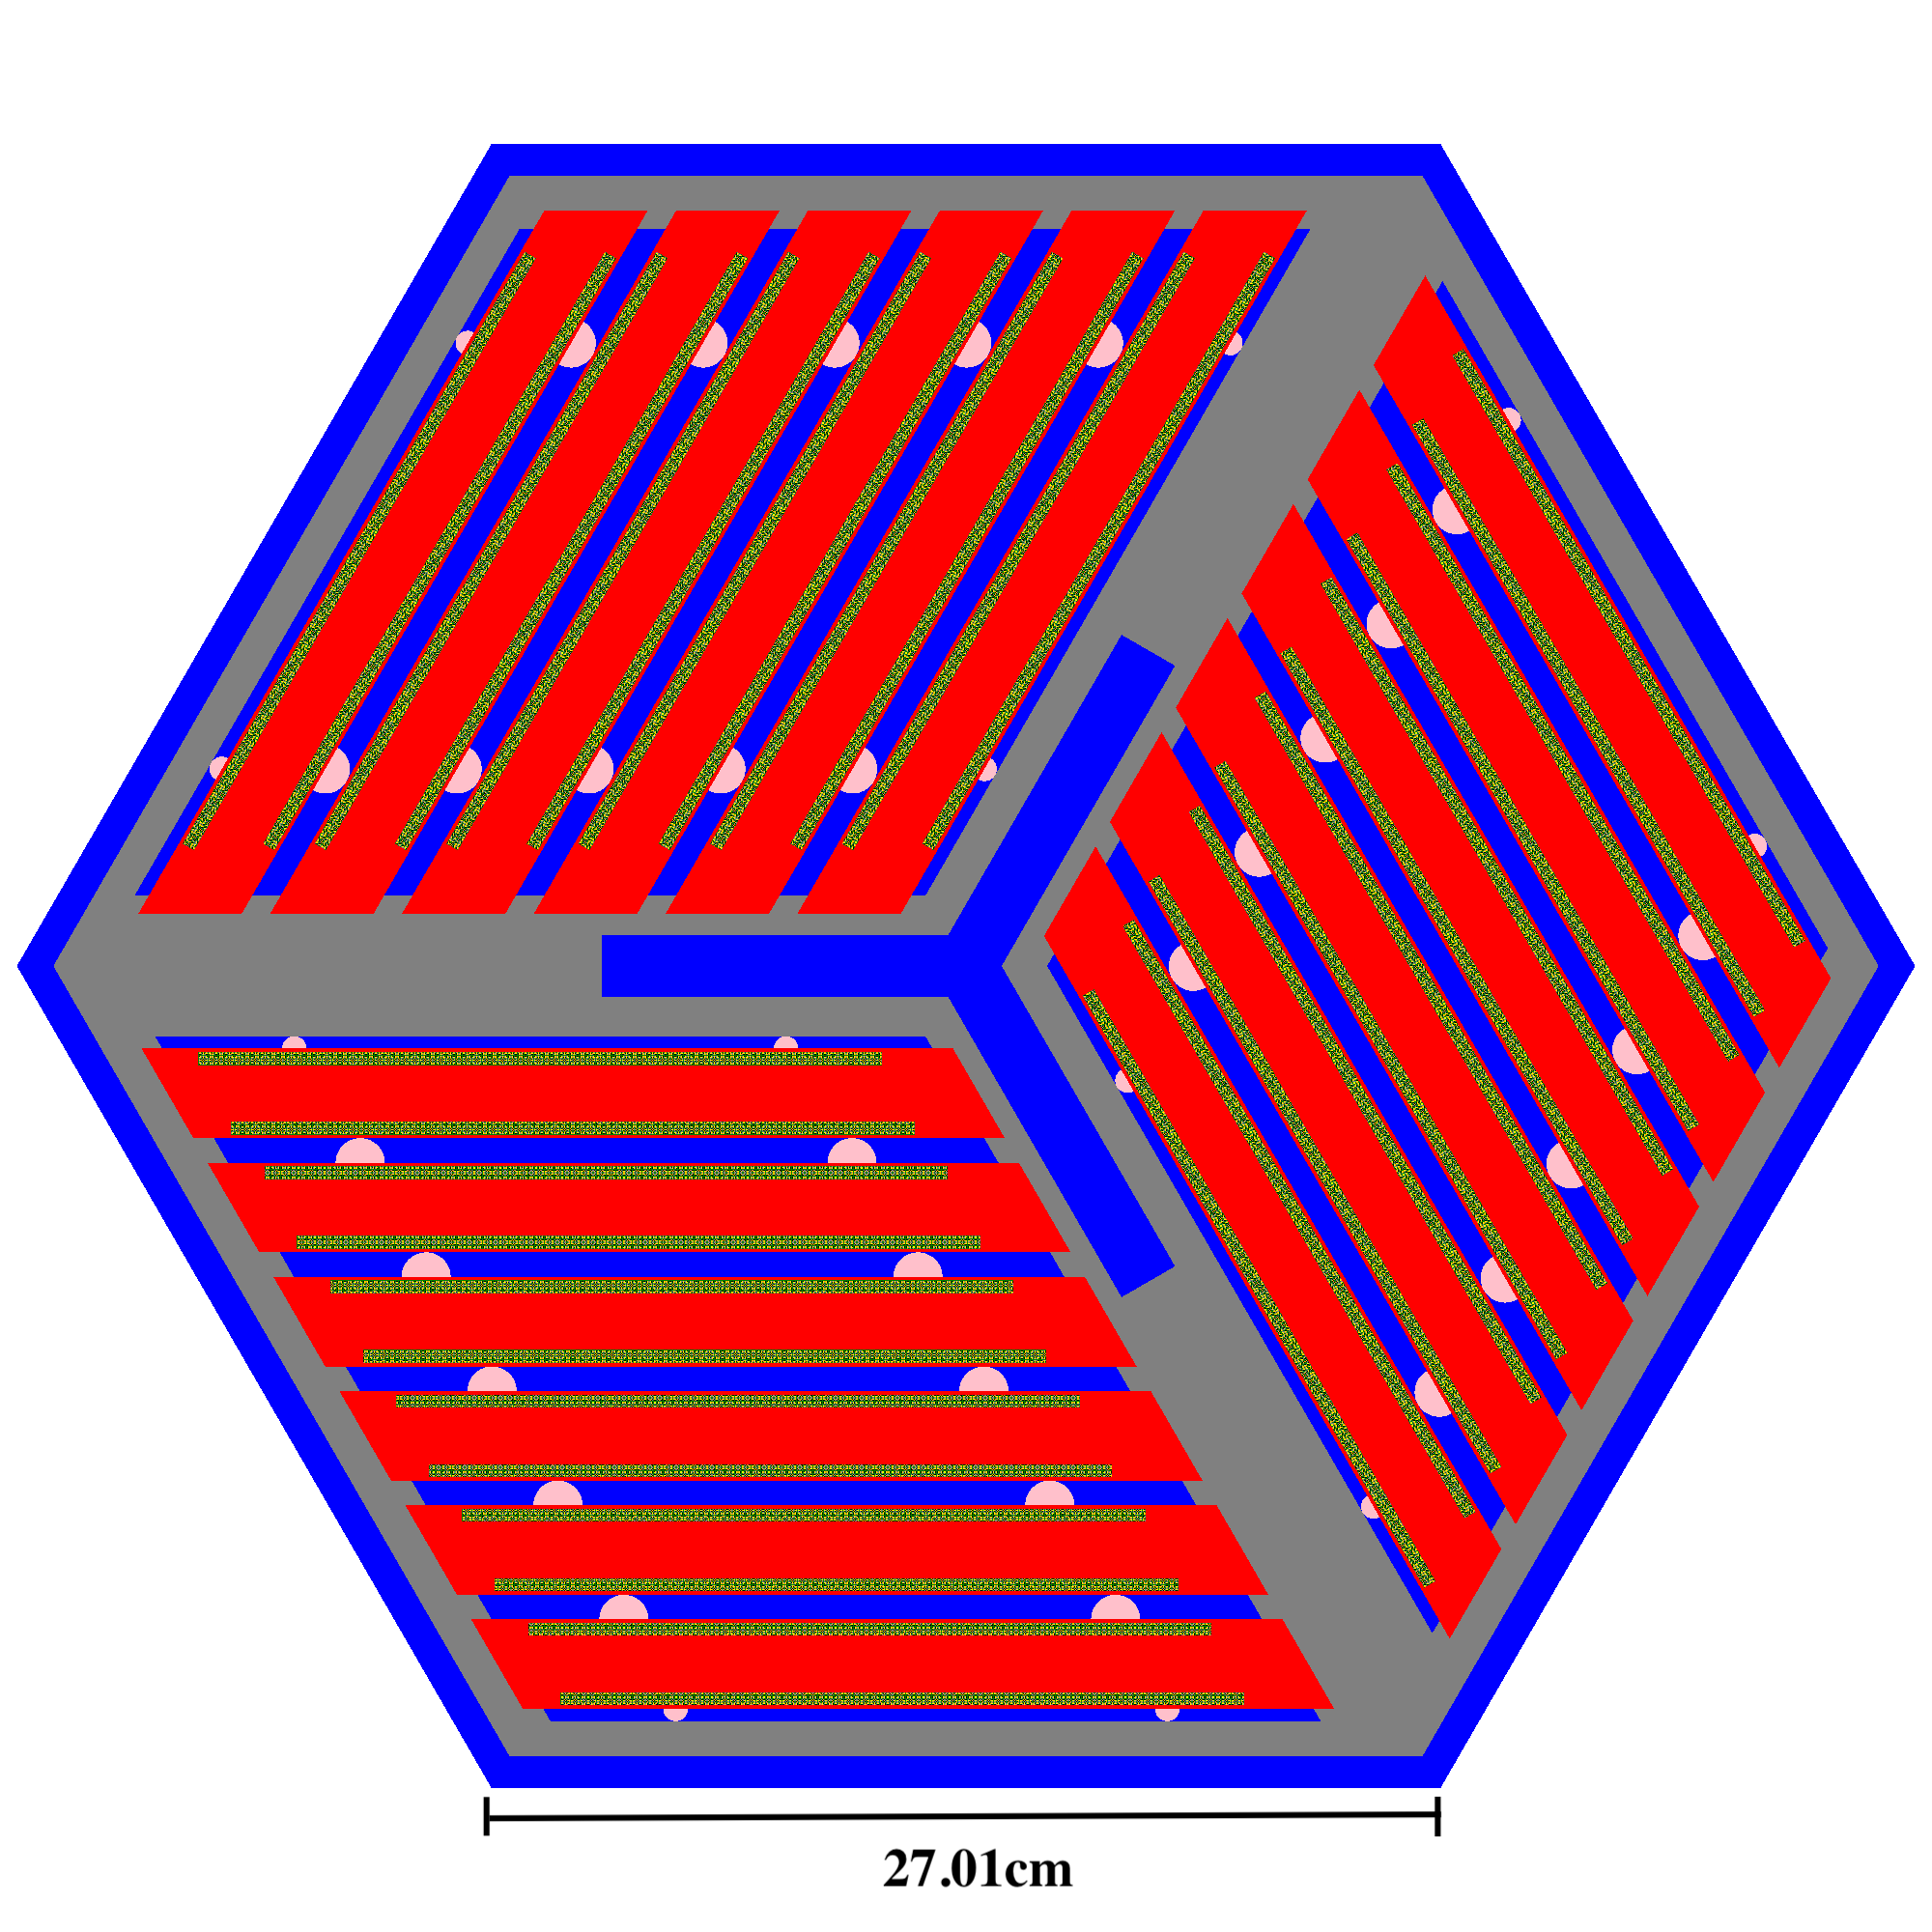
\includegraphics[width=0.49\linewidth]{../docs/figures/ahtr-fuel-element.png} 
    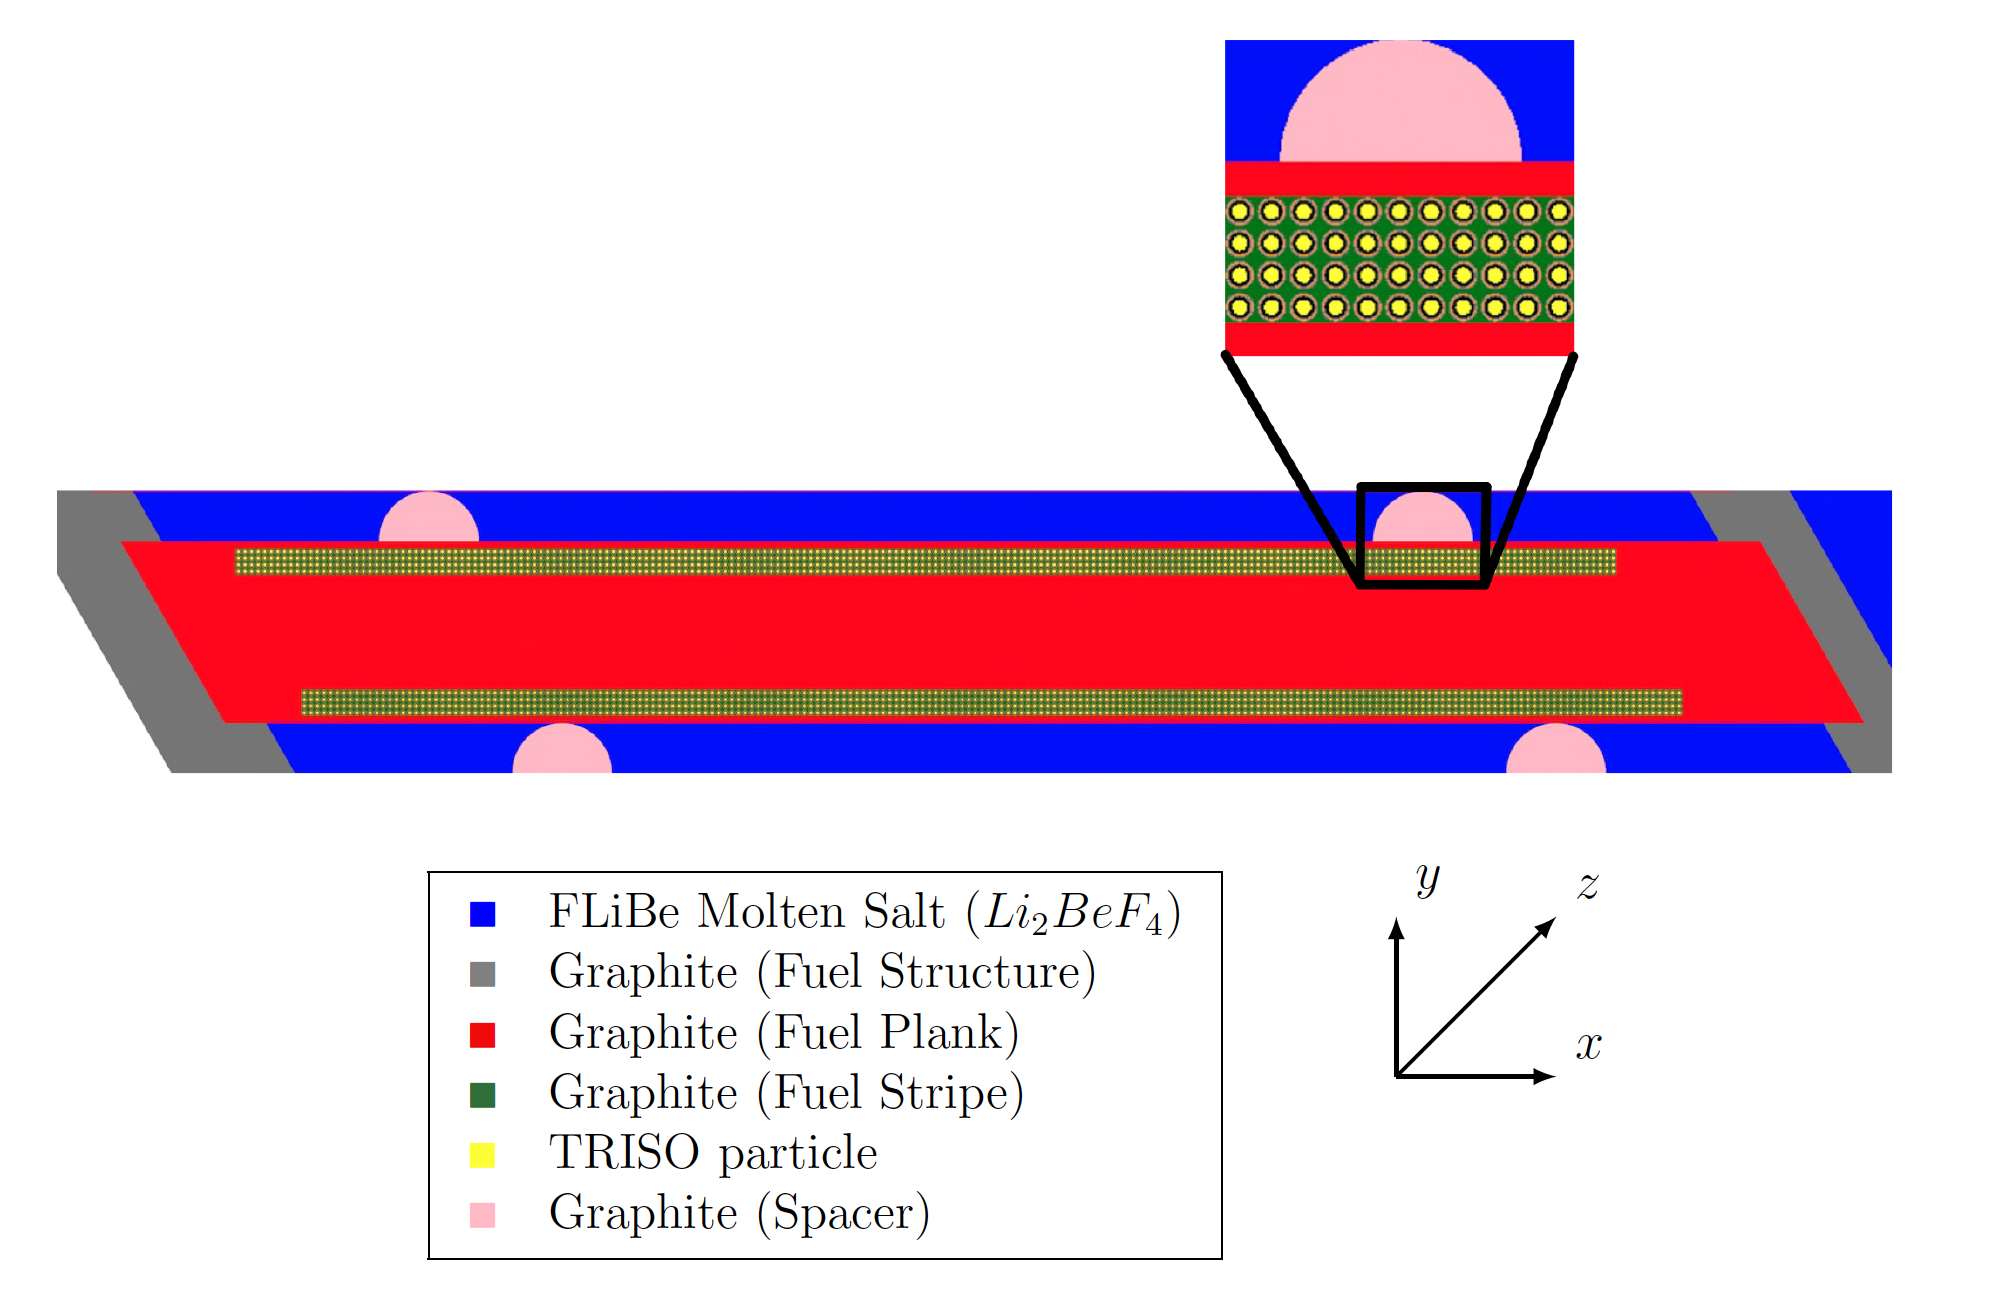
\includegraphics[width=0.49\linewidth]{figures/ahtr-plank.png}
    \caption{AHTR fuel assembly with 18 fuel plates arranged in 
    three diamond-shaped sectors, with a central Y-shaped and external channel 
    graphite structure.}
\end{figure}
\end{frame}

\begin{frame}
  \frametitle{FHR Benchmark}
  \begin{itemize}
    \item The AHTR's fuel geometry's triple heterogeneity results in
    complex reactor physics and significant modeling challenges
    \item In 2019 the OECD-NEA initiated a FHR benchmark exercise. Its objective 
    is to identify the applicability, accuracy, and practicality of the latest 
    methods and codes to assess the current state of the art for FHR simulation 
    and modeling
  \end{itemize}
  \begin{figure}[]
    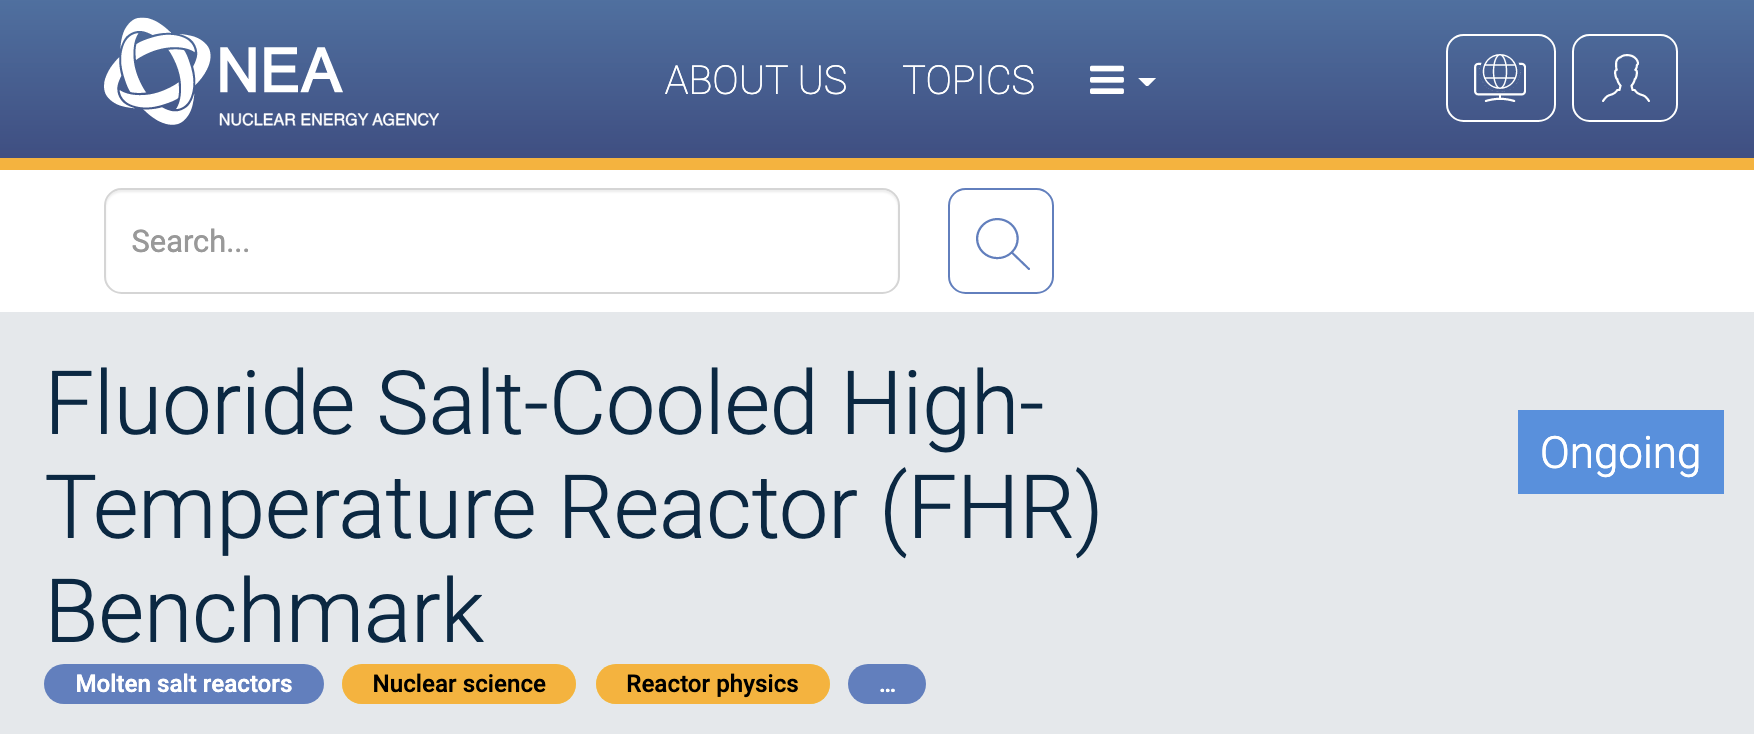
\includegraphics[width=0.7\linewidth]{figures/benchmark.png} 
    \caption{OECD NEA's FHR Benchmark \cite{petrovic_benchmark_2021}.}
\end{figure}
\end{frame}

\subsection{Objectives: AHTR Model Development}
\begin{frame}
  \frametitle{Research Objectives: AHTR Model Development}
  \begin{block}{Technical Gap}
      The triple heterogeneity introduced by the geometrically complex 
      fuel assembly design makes accurate reactor physics simulations challenging. 
  \end{block}
  \begin{block}{Research Objectives: AHTR Model Development}
    \begin{itemize}
      \item Further our understanding of the AHTR design's complexities 
      through neutronics and thermal-hydraulics modeling
      \item Participate in the OECD-NEA's FHR Benchmark 
    \end{itemize}
  \end{block}
  \begin{block}{Link to Reactor Optimization for Non-conventional Designs}
  \begin{itemize}
    \item By participating in the benchmark, I ensure an accurate AHTR base model
    \item Thus, I can expect accurate answers for the optimized AHTR designs
  \end{itemize}
  \end{block}
\end{frame}
\subsection{Background: Reactor optimization for non-conventional designs}
\begin{frame}
    \frametitle{3D Printing a Nuclear Reactor?}
    \begin{block}{Impact of Additive Manufacturing Technology Advancements on 
        Reactor Design Optimization}
        \begin{itemize}
            \item Leveraging additive manufacturing enables us to surpass classical 
            manufacturing constraints and optimize for arbitrary geometries and parameters 
            such as non-uniform channel shapes, and inhomogeneous fuel distribution 
            throughout the core
            \item Wide-spread adoption of additive manufacturing methods in the nuclear industry 
            could drastically reduce reactor fabrication costs and deployment timelines 
            and improve reactor safety
          \end{itemize}
    \end{block}
  \end{frame}

  \begin{frame}
    \frametitle{Evolutionary Algorithm Optimization}
    \begin{block}{Evolutionary Algorithms for Reactor Design Optimization}
    \begin{minipage}[c]{0.6\textwidth}
        \begin{itemize}
            \item We can leverage evolutionary algorithm optimization to 
            explore the large design space enabled by 3D printing to find global 
            optimal designs
            \item Evolutionary algorithms have proven successful in optimizing 
            multi-objective problems as they can find solutions at the global 
            optimum and can be run in parallel
            \item Evolutionary algorithms imitate natural selection to evolve solutions 
            \end{itemize}
  \end{minipage}\hfill
  \begin{minipage}[c]{0.4\textwidth}
    \centering
    \begin{figure}
      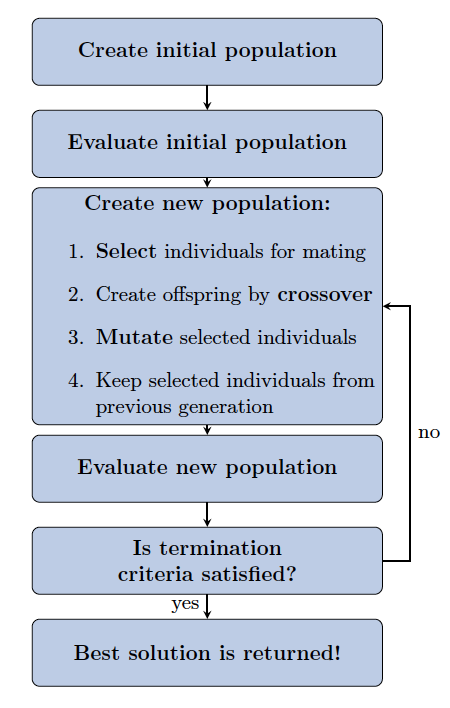
\includegraphics[width=0.8\linewidth]{figures/ea-flow.png} 
      \caption{Evolutionary algorithm flow \cite{renner_genetic_2003}. }
    \end{figure}
  \end{minipage}
  \end{block}
  \end{frame}
    
\subsection{Objectives: Reactor optimization for non-conventional designs}
\begin{frame}
    \frametitle{Research Objectives: AHTR optimization for non-conventional designs}
    \begin{block}{Technical Gap}
      \begin{itemize}
        \item Optimization tools for generating new reactor designs enabled by
        3D printing do not exist
        \item Reactor optimization for non-conventional geometries and parameters 
        has not been done 
      \end{itemize}
    \end{block}
    \begin{block}{Research Objectives: AHTR optimization for non-conventional designs}
        \begin{itemize}
            \item Develop an open-source tool that applies evolutionary algorithms with established 
            nuclear software to optimize reactor design
            \item Demonstrate successful application of the optimization tool 
            for single and multi-objective AHTR optimization of 
            non-conventional geometries and fuel distribution
        \end{itemize}
    \end{block}
  \end{frame}

\subsection{Summary}
\begin{frame}
    \frametitle{Summary}
    \textbf{Additive manufacturing could radically transform reactor design.}
    \begin{block}{Research Objectives: AHTR Model Development}
        \begin{itemize}
            \item Further our understanding of the AHTR design's complexities 
            through neutronics and thermal-hydraulics modeling
            \item Participate in the OECD-NEA's FHR Benchmark
        \end{itemize}
    \end{block}

    \begin{block}{Research Objectives: Reactor optimization for non-conventional designs}
        \begin{itemize}
            \item Develop a tool that applies evolutionary algorithms with established 
            nuclear software to optimize reactor design
            \item Demonstrate successful implementation of the optimization tool 
            with OpenMC for single and multi-objective AHTR optimization of 
            non-conventional geometries and fuel distribution
        \end{itemize}
    \end{block}
\end{frame}

\section{AHTR Model Development}
\subsection{FHR Benchmark Specifications}
\begin{frame}
    \frametitle{FHR Benchmark Specifications}
    \begin{itemize}
        \item UIUC participates in the benchmark with OpenMC and using the ENDF/B-VII.1 material 
        cross section library
    \end{itemize}
    \vspace{-0.2cm}
    \begin{table}
        \caption{OECD NEA's FHR Benchmark Phases 
        \cite{petrovic_benchmark_2021}.}
        \vspace{-0.25cm}
        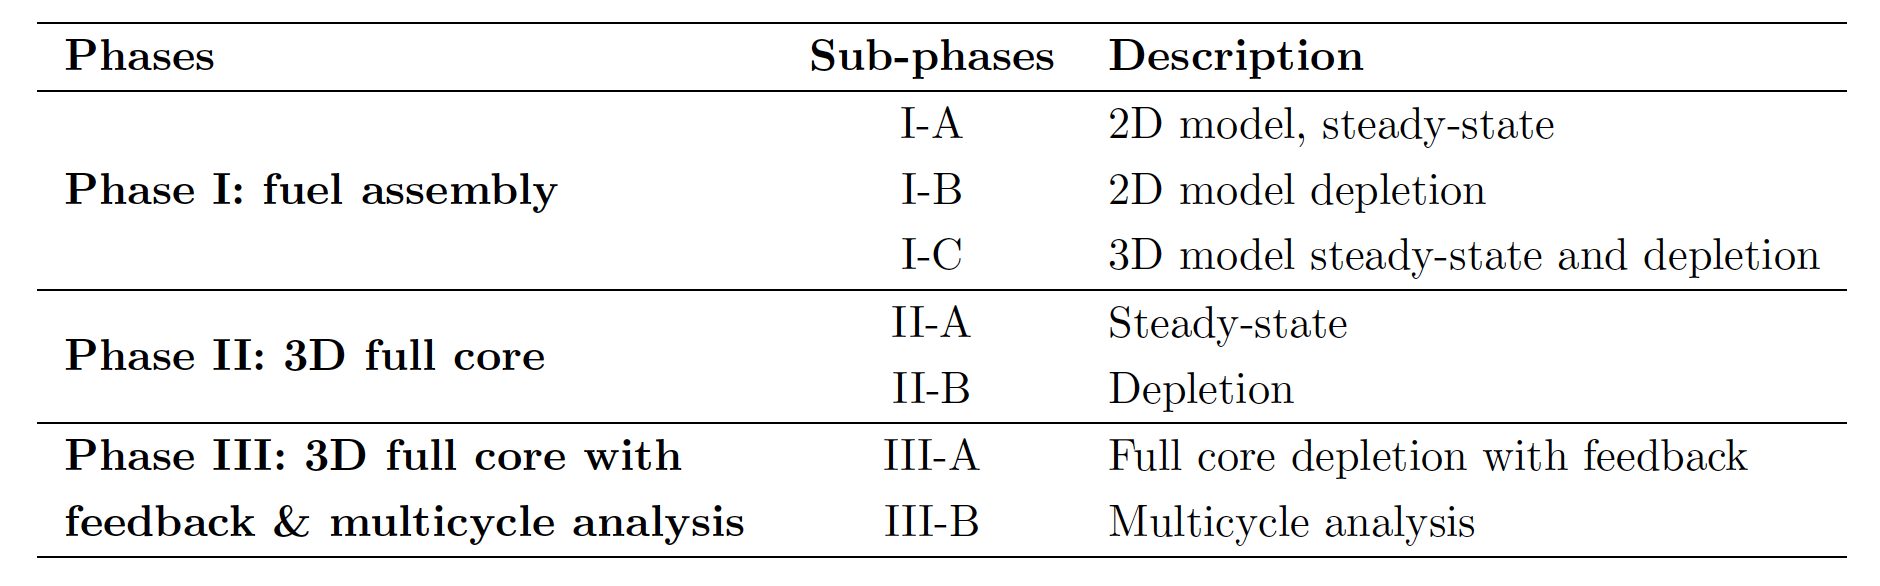
\includegraphics[width=0.7\linewidth]{figures/benchmark-phases.png} 
    \end{table}
    \vspace{-0.3cm}
    \begin{figure}[]
        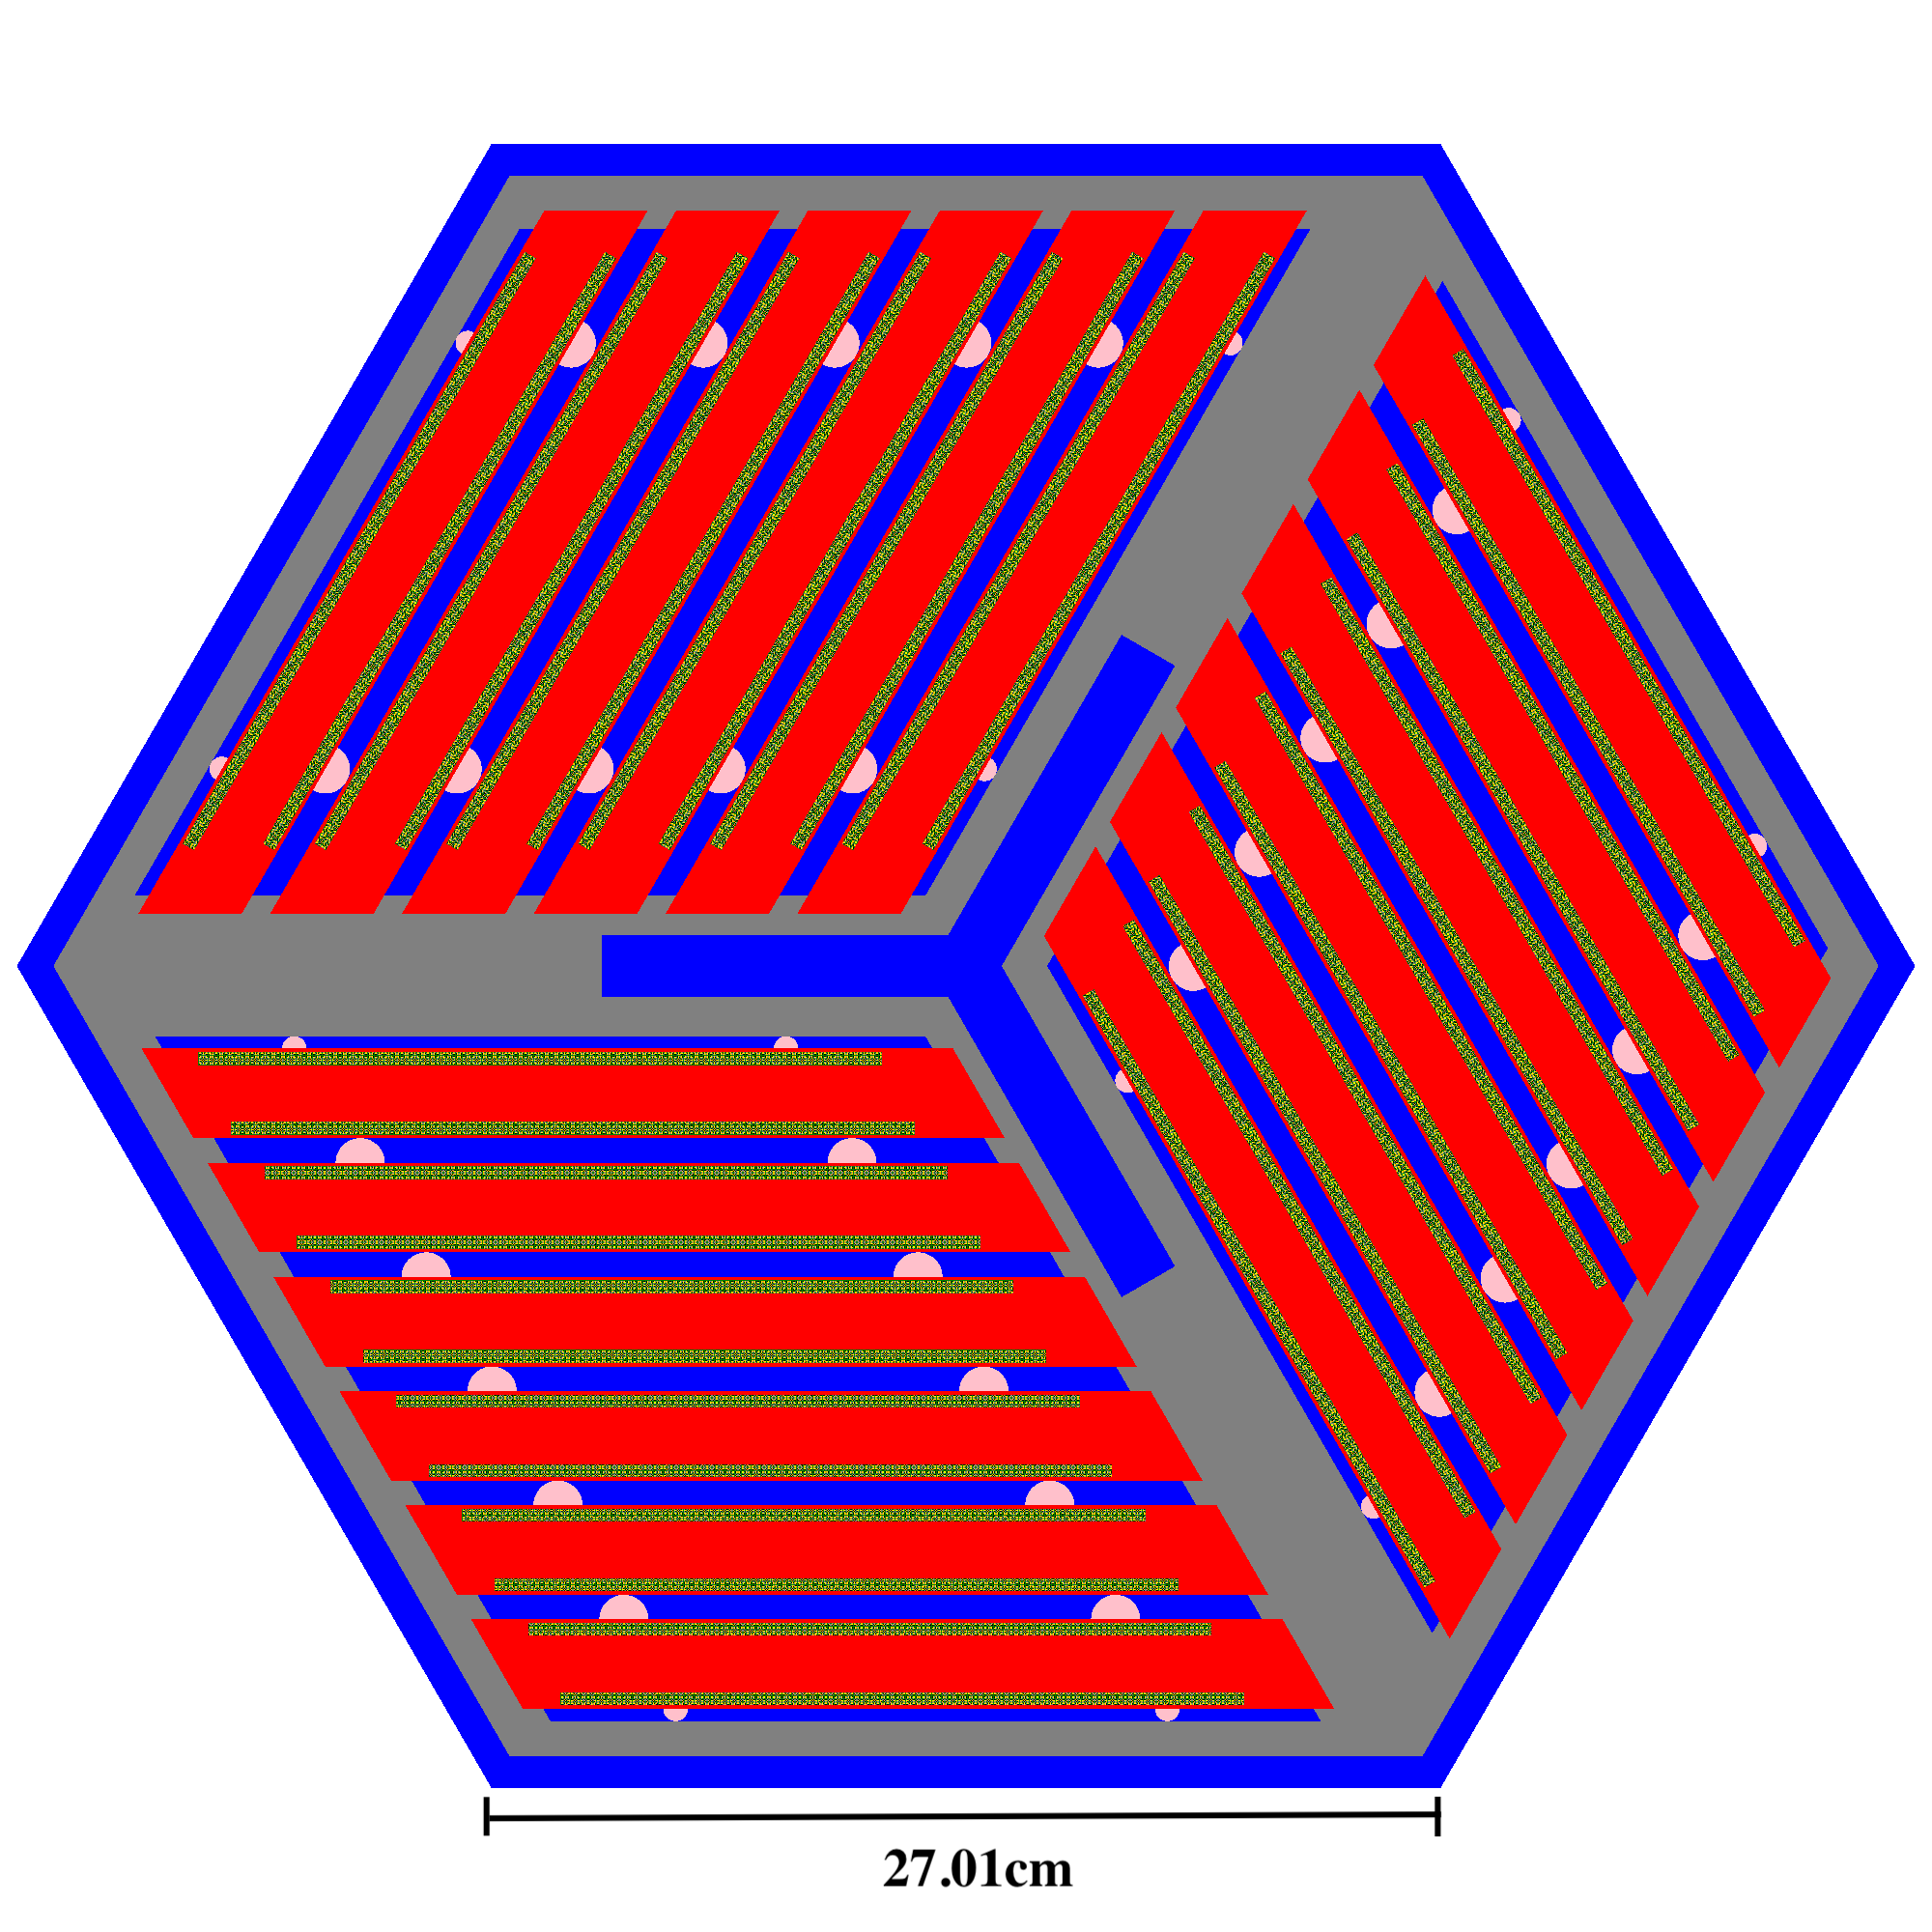
\includegraphics[width=0.27\linewidth]{../docs/figures/ahtr-fuel-element.png} 
        \vspace{-0.2cm}
        \caption{AHTR fuel assembly.}
    \end{figure}
\end{frame}

\begin{frame}
    \frametitle{FHR Benchmark Specifications}
    \begin{itemize}
        \item Only Phase I-A and I-B specifications have been released 
        \item Benchmark participants must produce the following results for 
        the 9 cases: $k_{eff}$, reactivity coefficients ($\beta_{eff}$, 
        $\alpha_D$, $\alpha_{T, FliBe}$, $\alpha_M$), fission source distribution, 
        neutron flux distribution, fuel assembly averaged neutron spectrum
    \end{itemize}
    \vspace{-0.25cm}
    \begin{table}
        \caption{Description of the \acrlong{FHR} benchmark Phase I-A cases 
        \vspace{-0.25cm}
        \cite{noauthor_fluoride_nodate}.}
        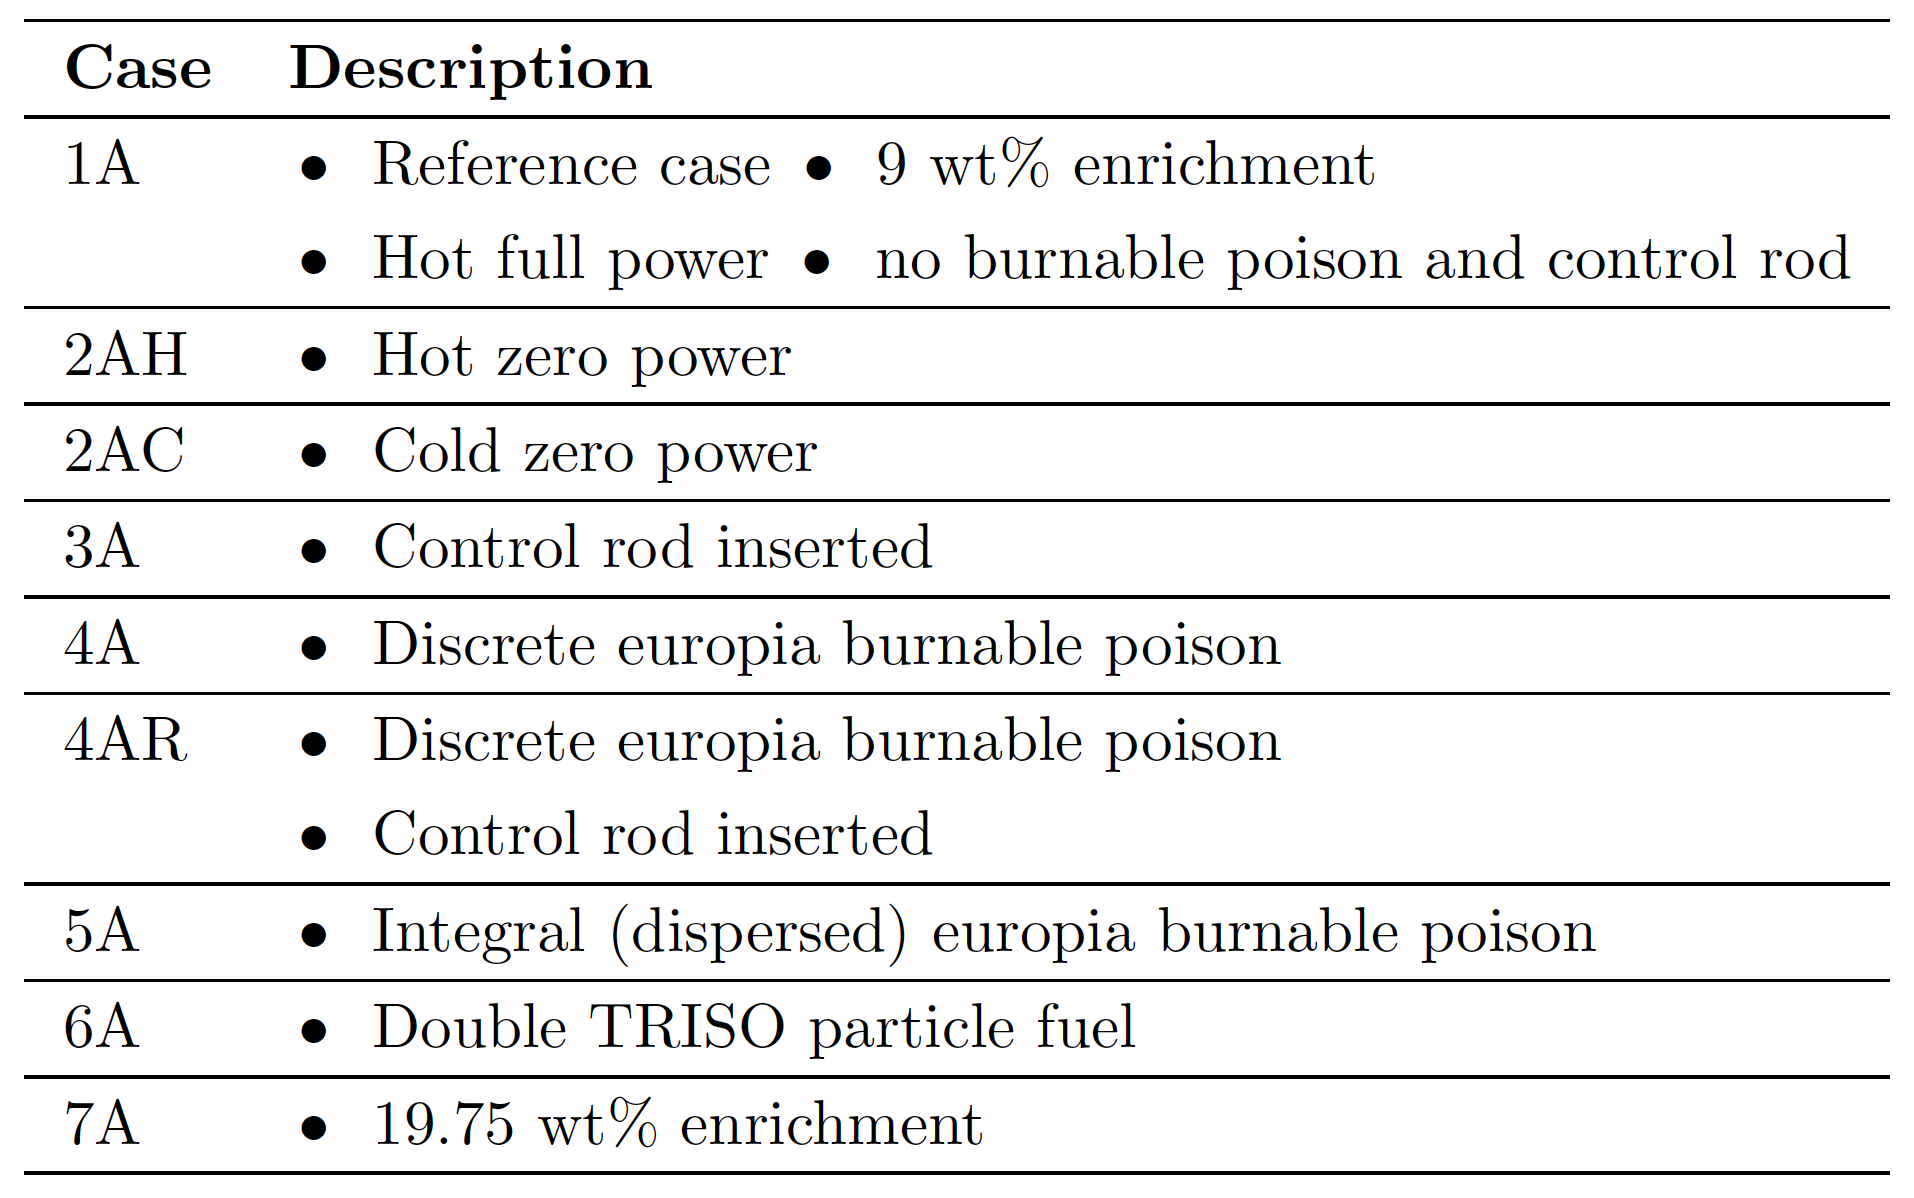
\includegraphics[width=0.6\linewidth]{figures/benchmark-cases.png} 
    \end{table}
\end{frame}
\subsection{Results}

\section{AHTR Optimization}
\subsection{Methodology}

\section{Conclusion}

%\input{acks}
%%--------------------------------%%
%%--------------------------------%%
\begin{frame}[allowframebreaks]
  \frametitle{References}
  \bibliographystyle{ieeetr}
  {\footnotesize \bibliography{../docs/2022-chee-dissertation.bib} }

\end{frame}

%\section*{Appendix}
%\subsection*{Grad School Journey}
\begin{frame}
    \frametitle{Grad School Journey}
    \vspace{-0.2cm}
    \begin{figure}[]
        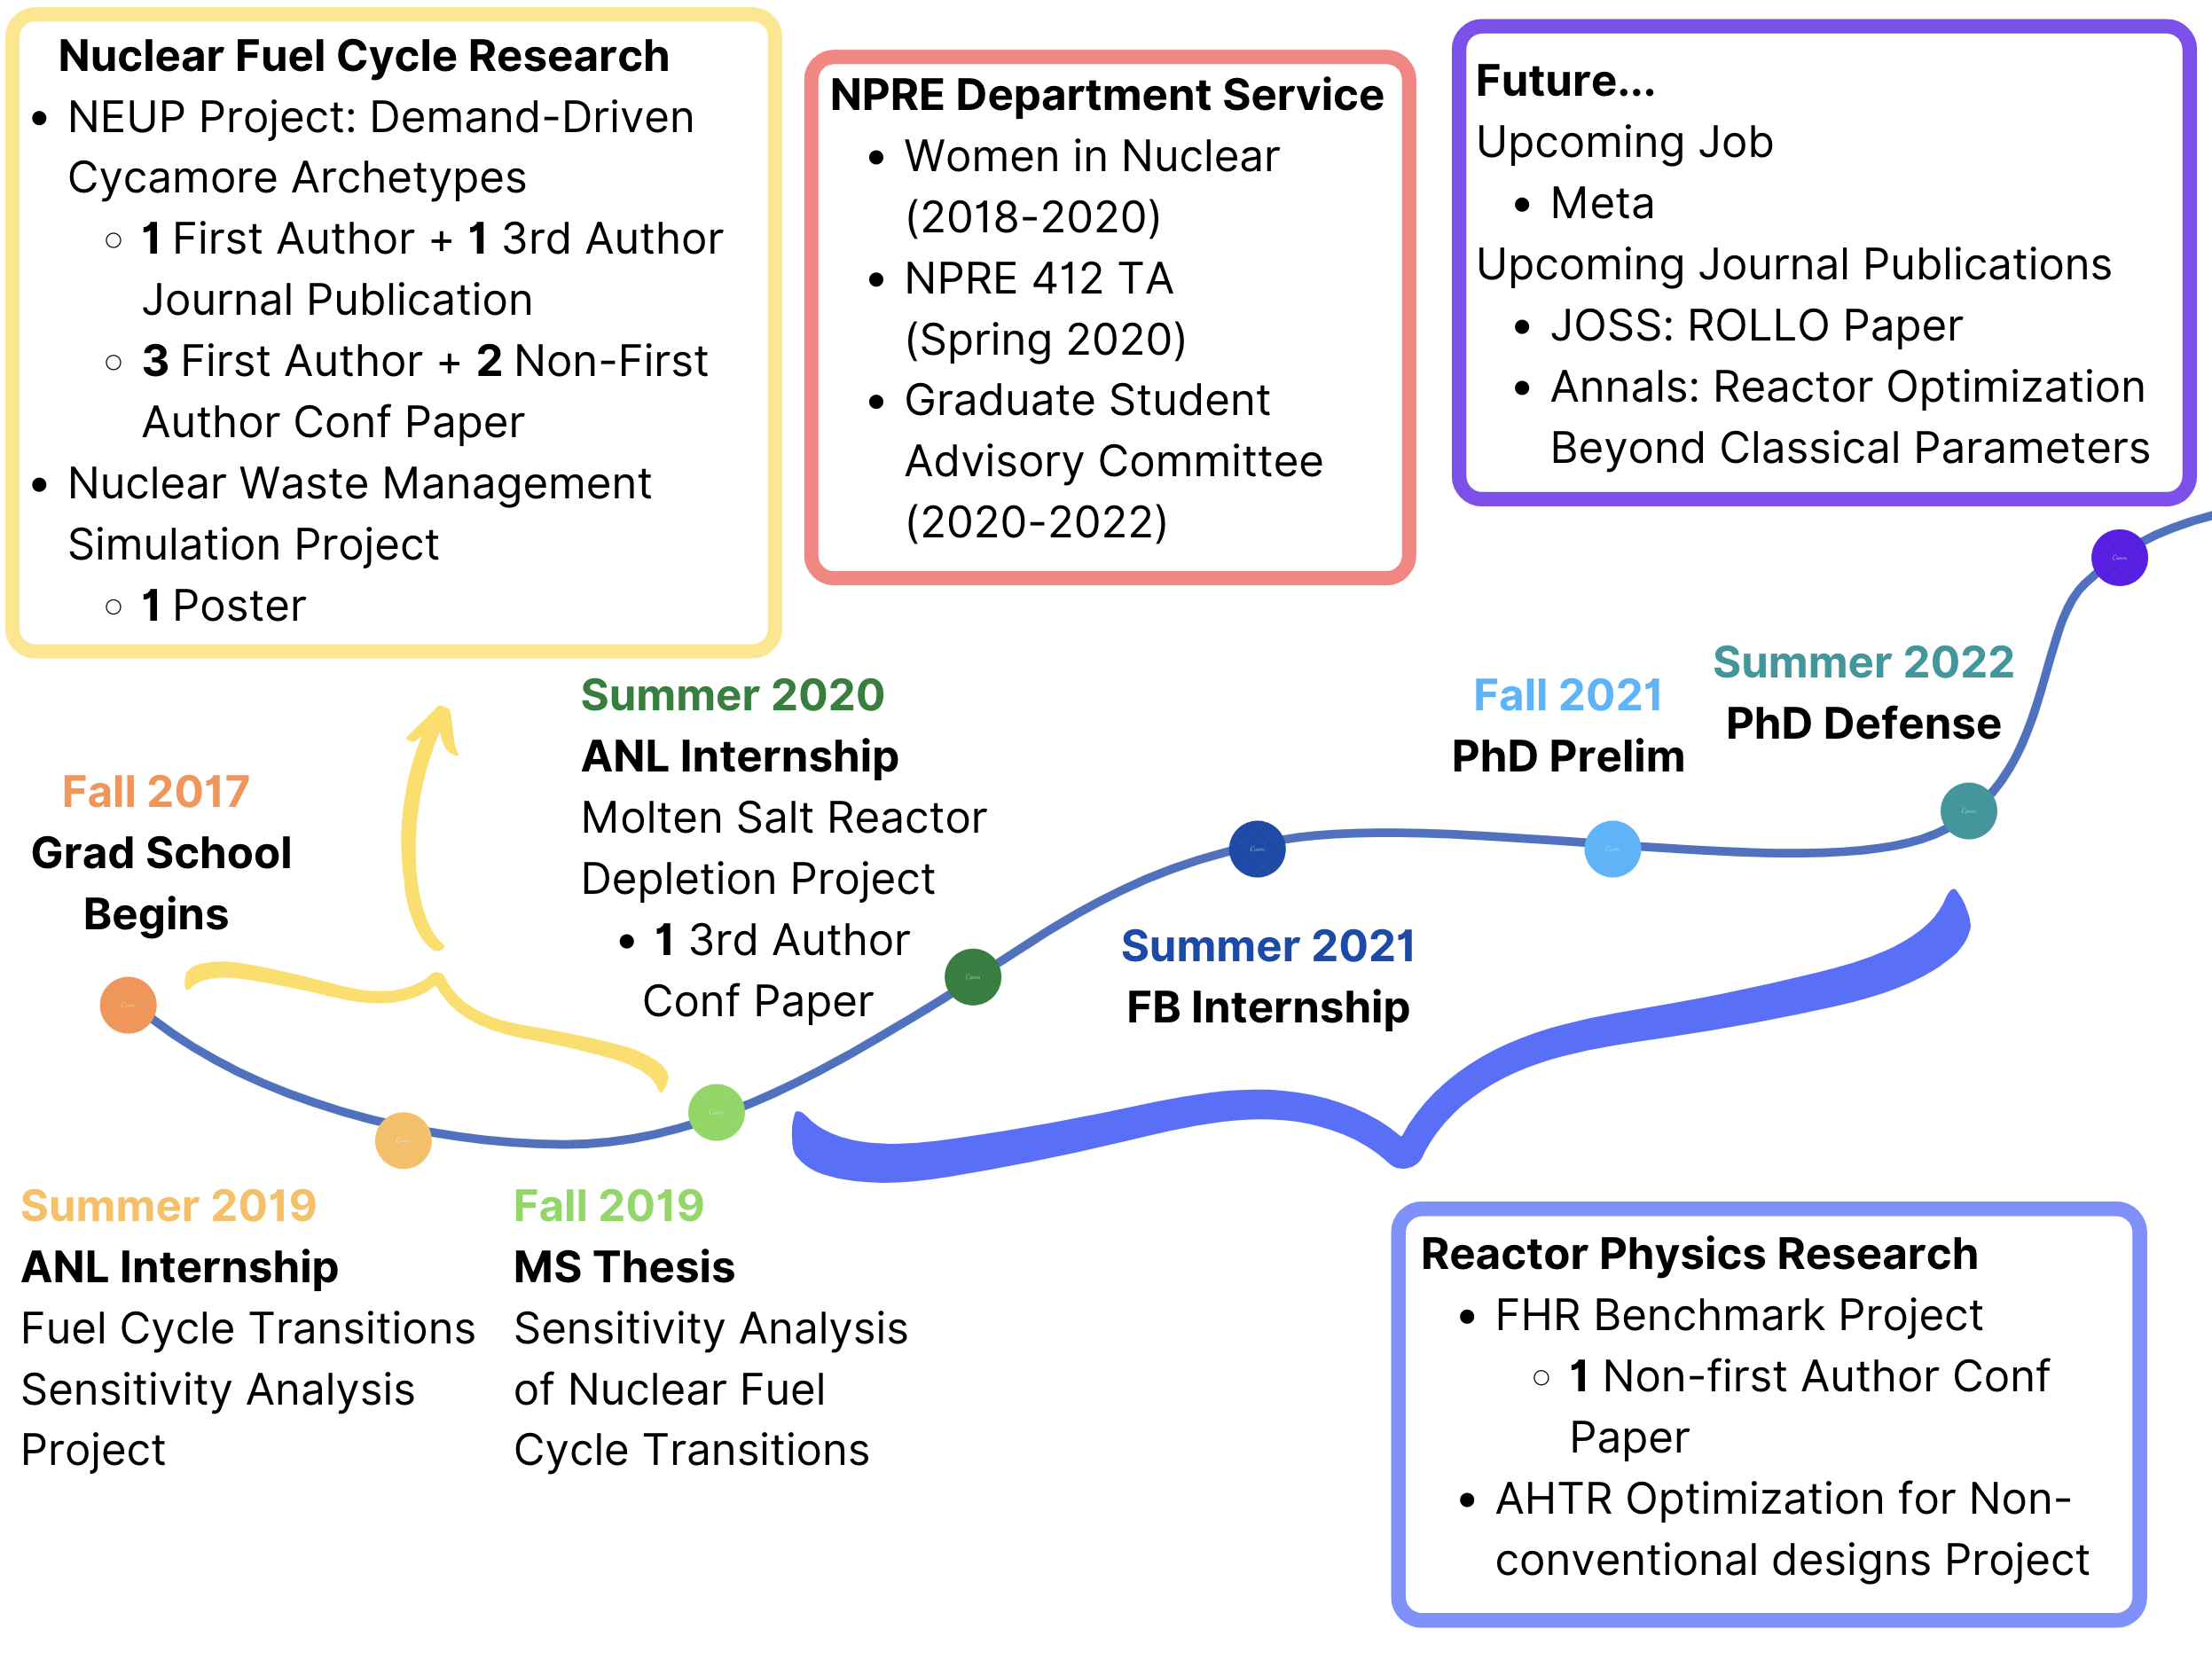
\includegraphics[width=0.9\linewidth]{figures/grad-school-journey.png} 
    \end{figure}
\end{frame}

\subsection*{Summary}
\begin{frame}
    \frametitle{Summary}
    \begin{columns}[t]
        \begin{column}{0.5\linewidth}
            \begin{block}{AHTR Model Development for the FHR Benchmark}
                \textbf{Results Presented} 
                \begin{itemize}
                    \item FHR benchmark Phase I-A and I-B results
                    \item AHTR full assembly temperature model 
                \end{itemize}

                Through participation in the FHR benchmark, this dissertation contributes to 
                \textbf{deepening our understanding of the promising \gls{AHTR} technology}.
            \end{block}
        \end{column}
        \begin{column}{0.5\linewidth}
            \begin{block}{ROLLO Tool Development and AHTR Non-Conventional Design Optimization}
                \textbf{Results Presented}
                \begin{itemize}
                    \item \acrfull{ROLLO} tool 
                    \item AHTR Optimization for heterogeneous fuel distributions and wavy 
                    coolant channels 
                \end{itemize}
                
                By designing the ROLLO tool and demonstrating its success in 
                optimization of the \gls{AHTR} beyond classical input parameters, this dissertation 
                contributes to \textbf{optimization tool development for reactors of the future}.
            \end{block}
        \end{column}
    \end{columns}
\end{frame}

\subsection*{FHR Benchmark Specifications}
\begin{frame}
    \frametitle{FHR Benchmark Specifications}
    UIUC participates in the benchmark with OpenMC and using the ENDF/B-VII.1 material 
    cross section library
    \vspace{-0.2cm}
    \begin{table}
        \caption{OECD NEA's FHR Benchmark Phases 
        \cite{petrovic_benchmark_2021}.}
        \vspace{-0.25cm}
        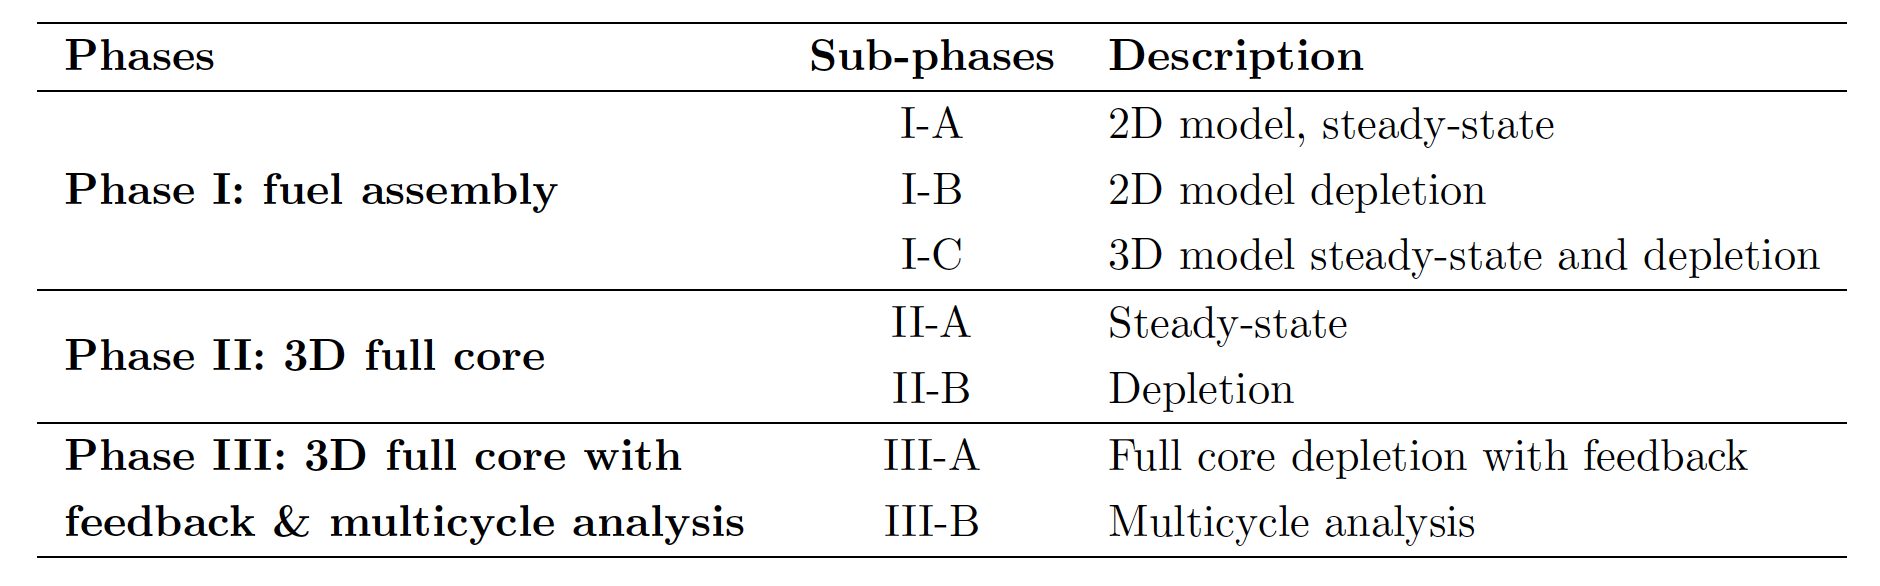
\includegraphics[width=0.7\linewidth]{figures/benchmark-phases.png} 
    \end{table}
    \vspace{-0.3cm}
    \begin{figure}[]
        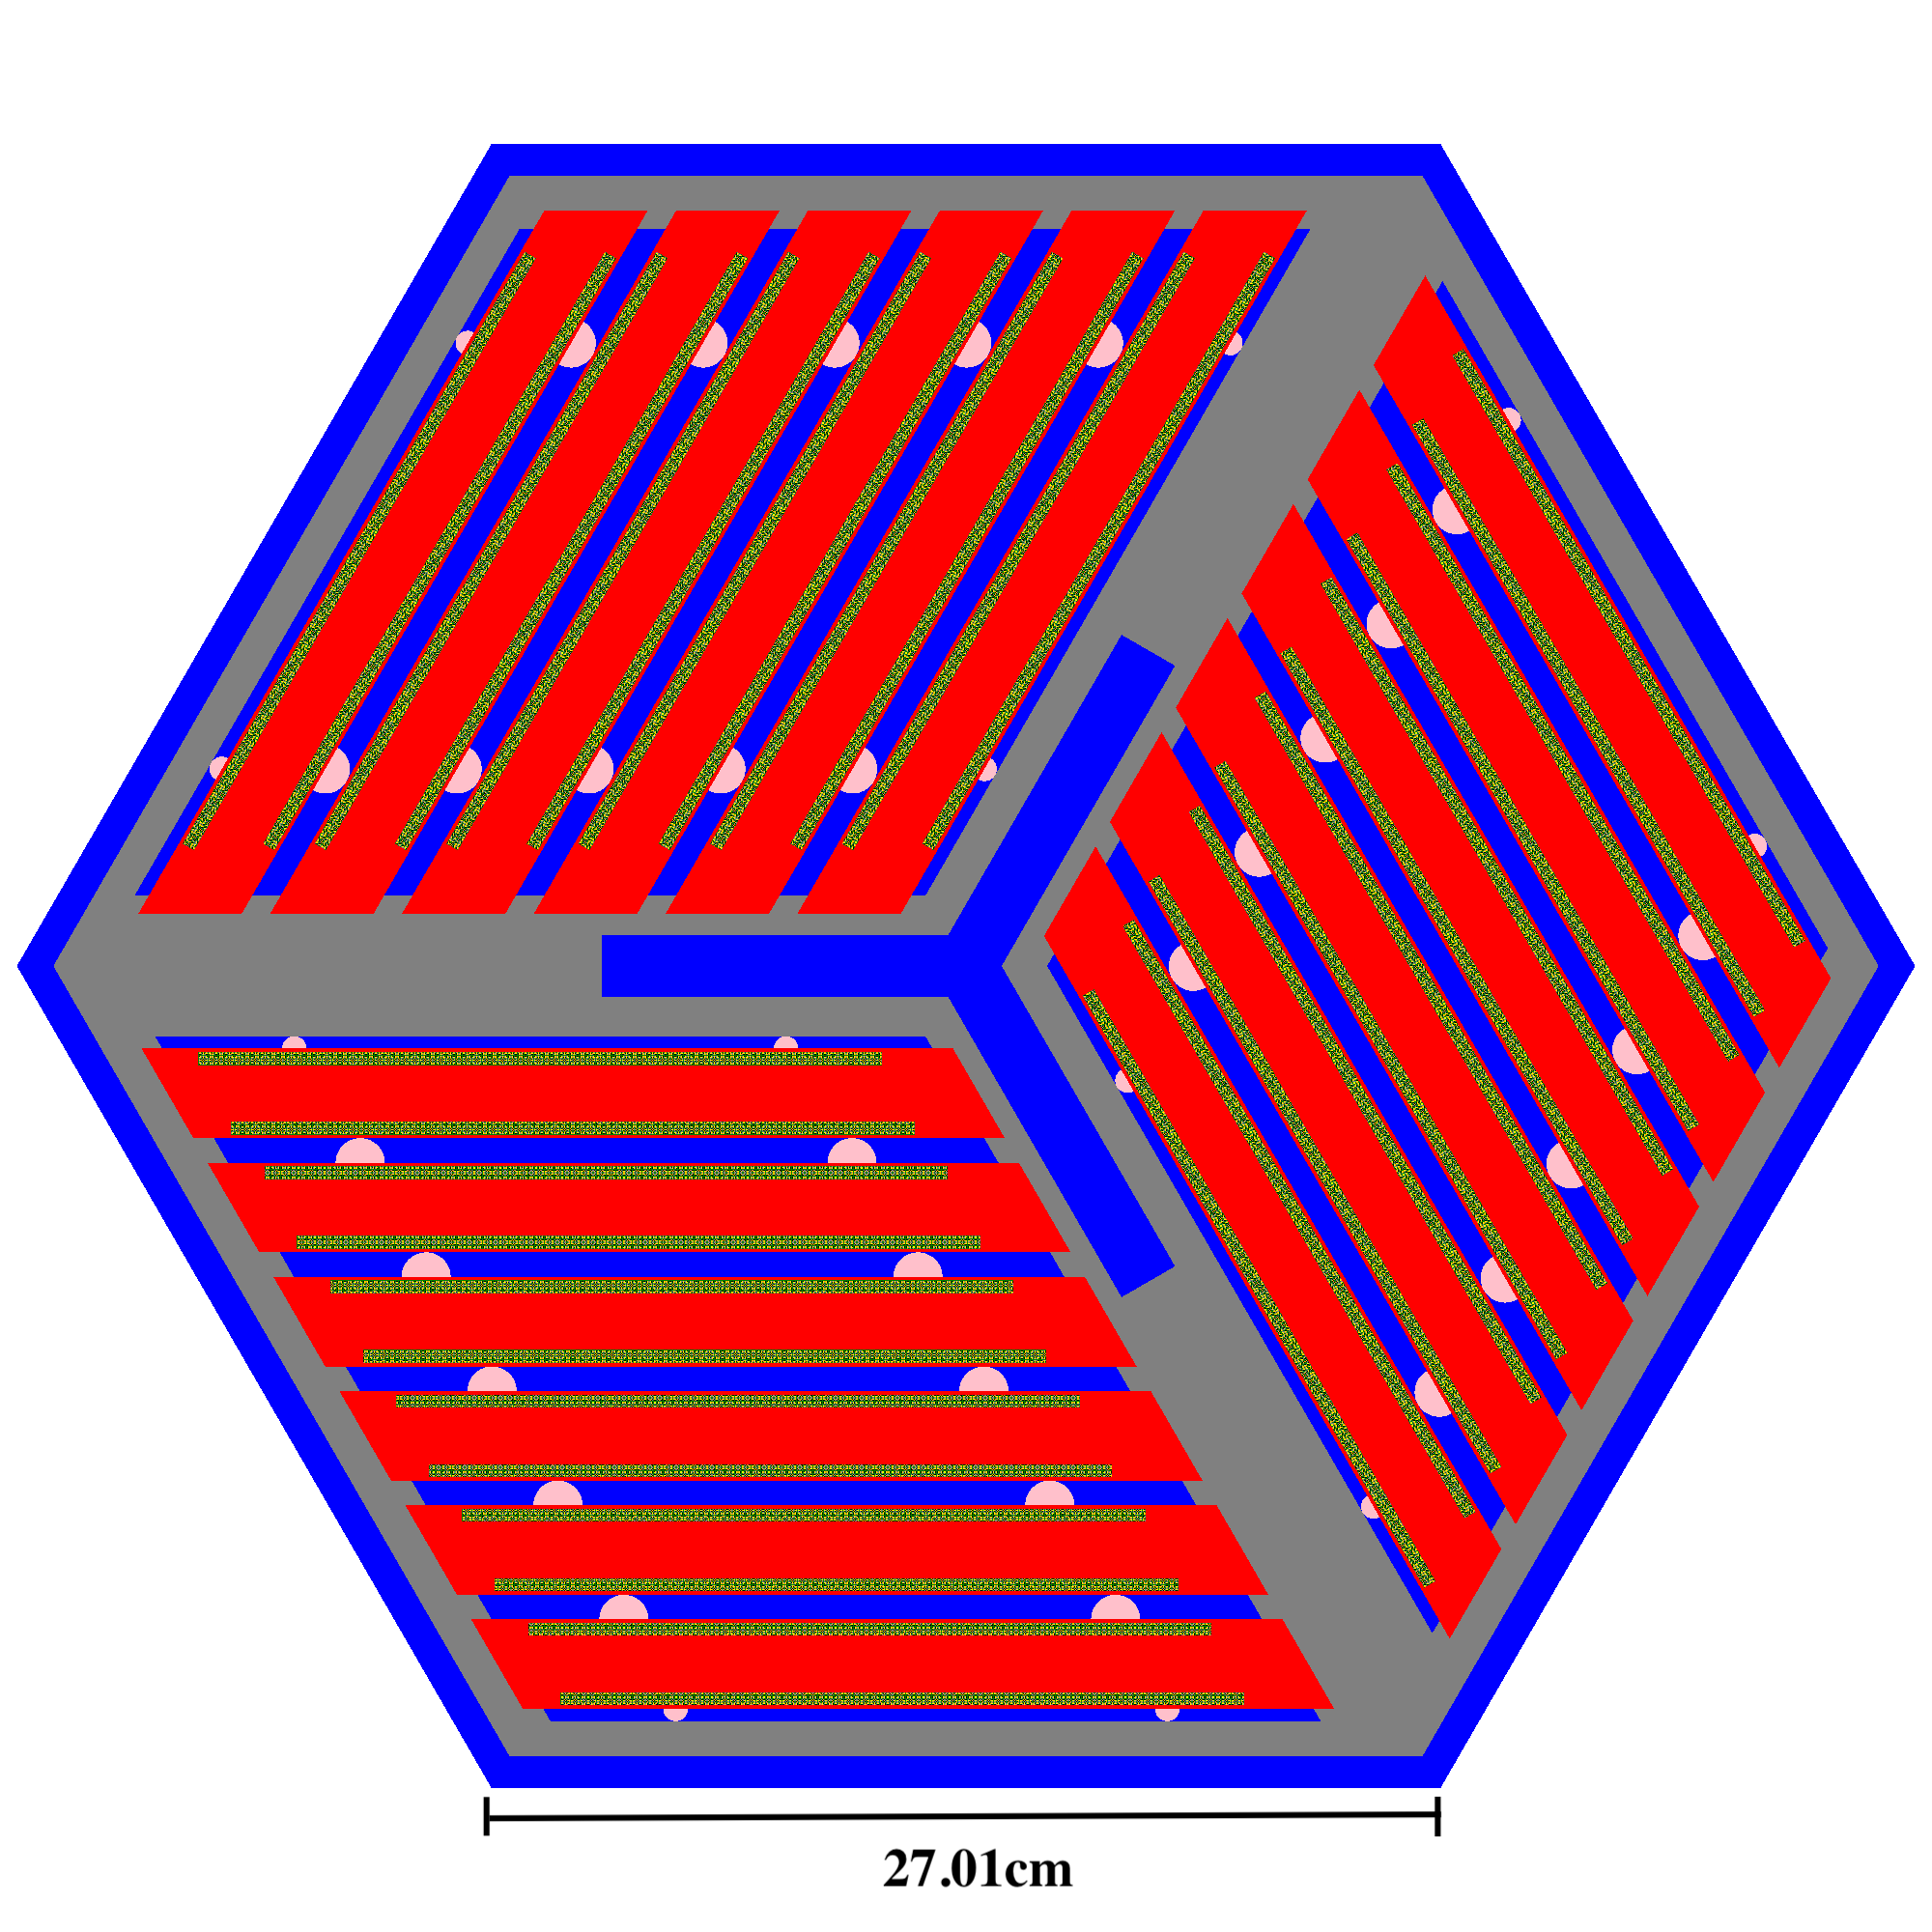
\includegraphics[width=0.27\linewidth]{../docs/figures/ahtr-fuel-element.png} 
        \vspace{-0.2cm}
        \caption{AHTR fuel assembly.}
    \end{figure}
\end{frame}

\begin{frame}
    \frametitle{FHR Benchmark Specifications}
    Only Phase I-A and I-B specifications have been released 
    \begin{table}
        \caption{Description of the \acrlong{FHR} benchmark Phase I-A cases 
        \vspace{-0.25cm}
        \cite{petrovic_benchmark_2021}.}
        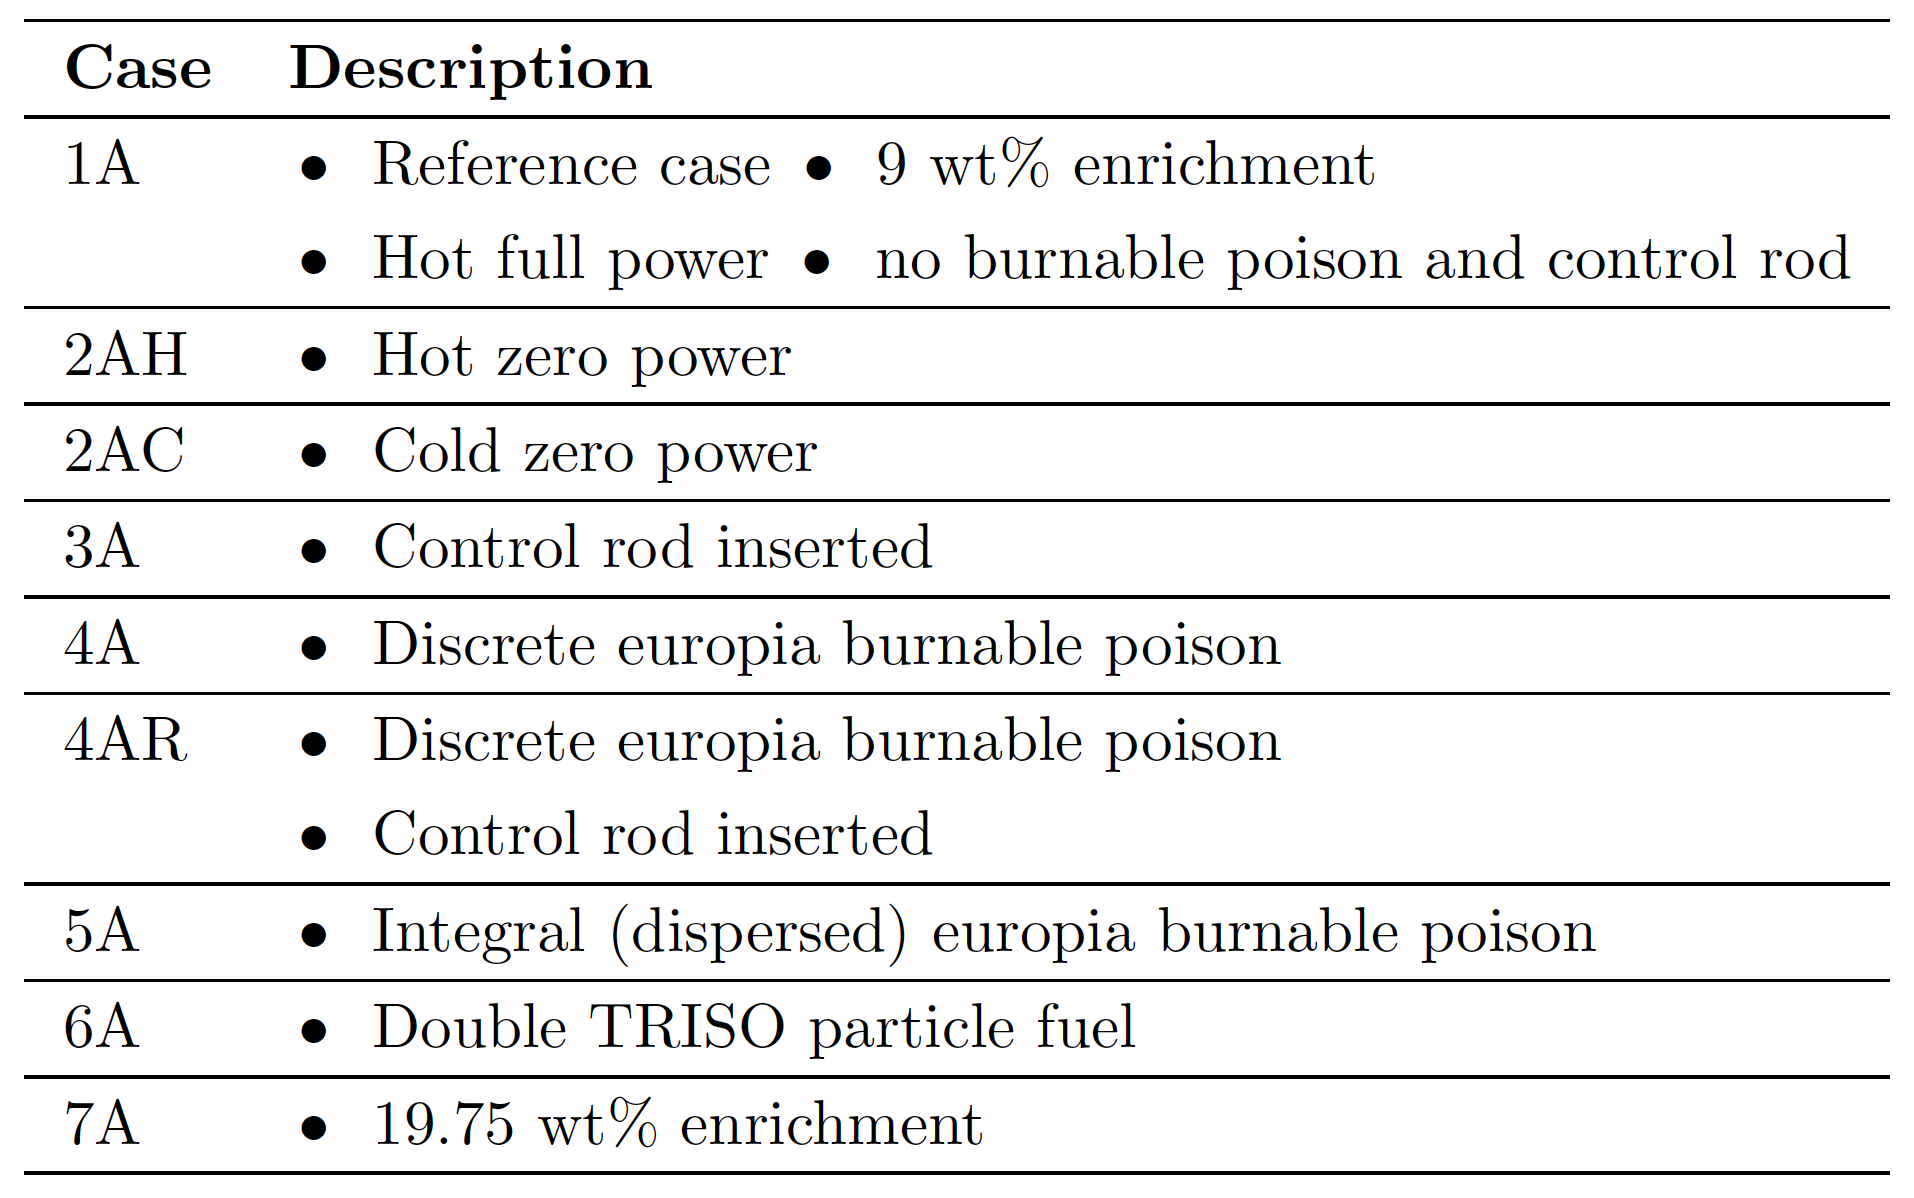
\includegraphics[width=0.6\linewidth]{figures/benchmark-cases.png} 
    \end{table}
    Benchmark participants must produce the following results for 
    the 9 cases: $k_{eff}$, reactivity coefficients ($\beta_{eff}$, 
    $\alpha_D$, $\alpha_{T, FliBe}$, $\alpha_M$), fission source distribution, 
    neutron flux distribution, fuel assembly averaged neutron spectrum
\end{frame}

\subsection*{Key Neutronics Parameters Verification}
\begin{frame}
    \frametitle{AHTR Temp Model $k_{eff}$ and Reactivity Coefficients Verification}
        \begin{table}
            \caption{$k_{eff}$ and reactivity comparison.}
            \vspace{-0.2cm}
            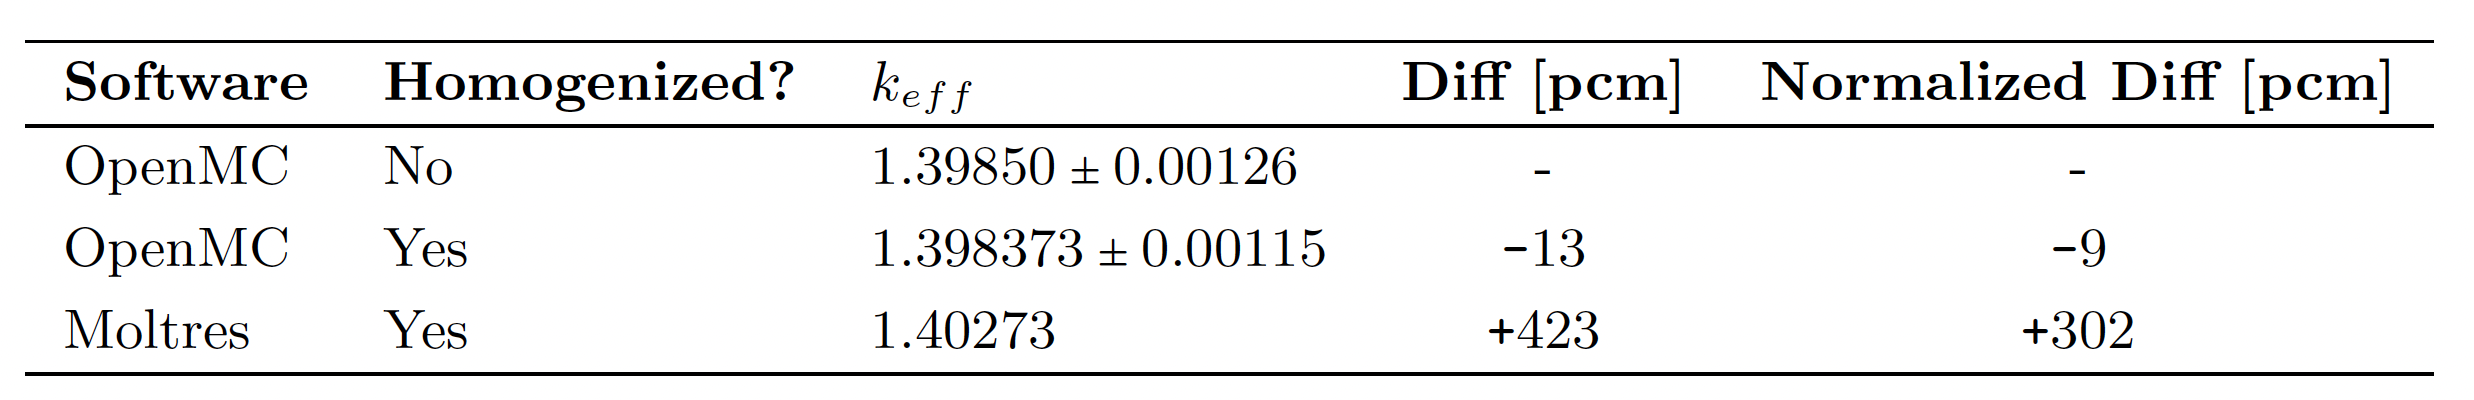
\includegraphics[width=0.9\linewidth]{figures/benchmark-keff.png}
        \end{table}
        The 13pcm $k_{eff}$ and 6pcm reactivity diff, between
        continuous and homogenized OpenMC simulations are within uncertainty, showing 
        that \textbf{selected spatial homogenizations and energy discretizations are 
        acceptable.}
        The Moltres simulation shows a 423pcm diff in $k_{eff}$ and 216pcm 
        diff in reactivity.
        \begin{table}
            \caption{Reactivity coefficients comparison.}
            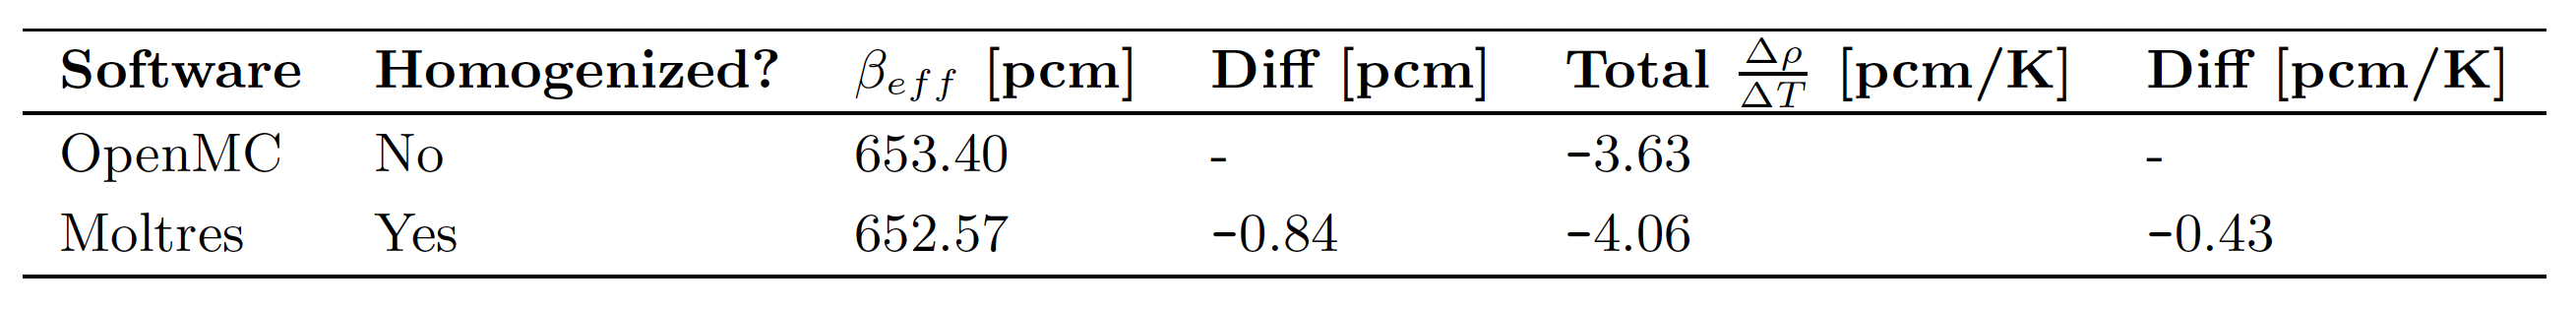
\includegraphics[width=0.85\linewidth]{figures/benchmark-coeff.png}
        \end{table}
        \textbf{Good agreement} for Moltres' delayed neutron fraction ($\beta_{eff}$) and 
        temperature reactivity feedback ($\frac{\Delta \rho}{\Delta T}$)
\end{frame}

\begin{frame}
    \frametitle{AHTR Temp Model Flux Verification}
    \begin{columns}
    \begin{column}{0.7\textwidth}
    \begin{figure}[]
        \centering
        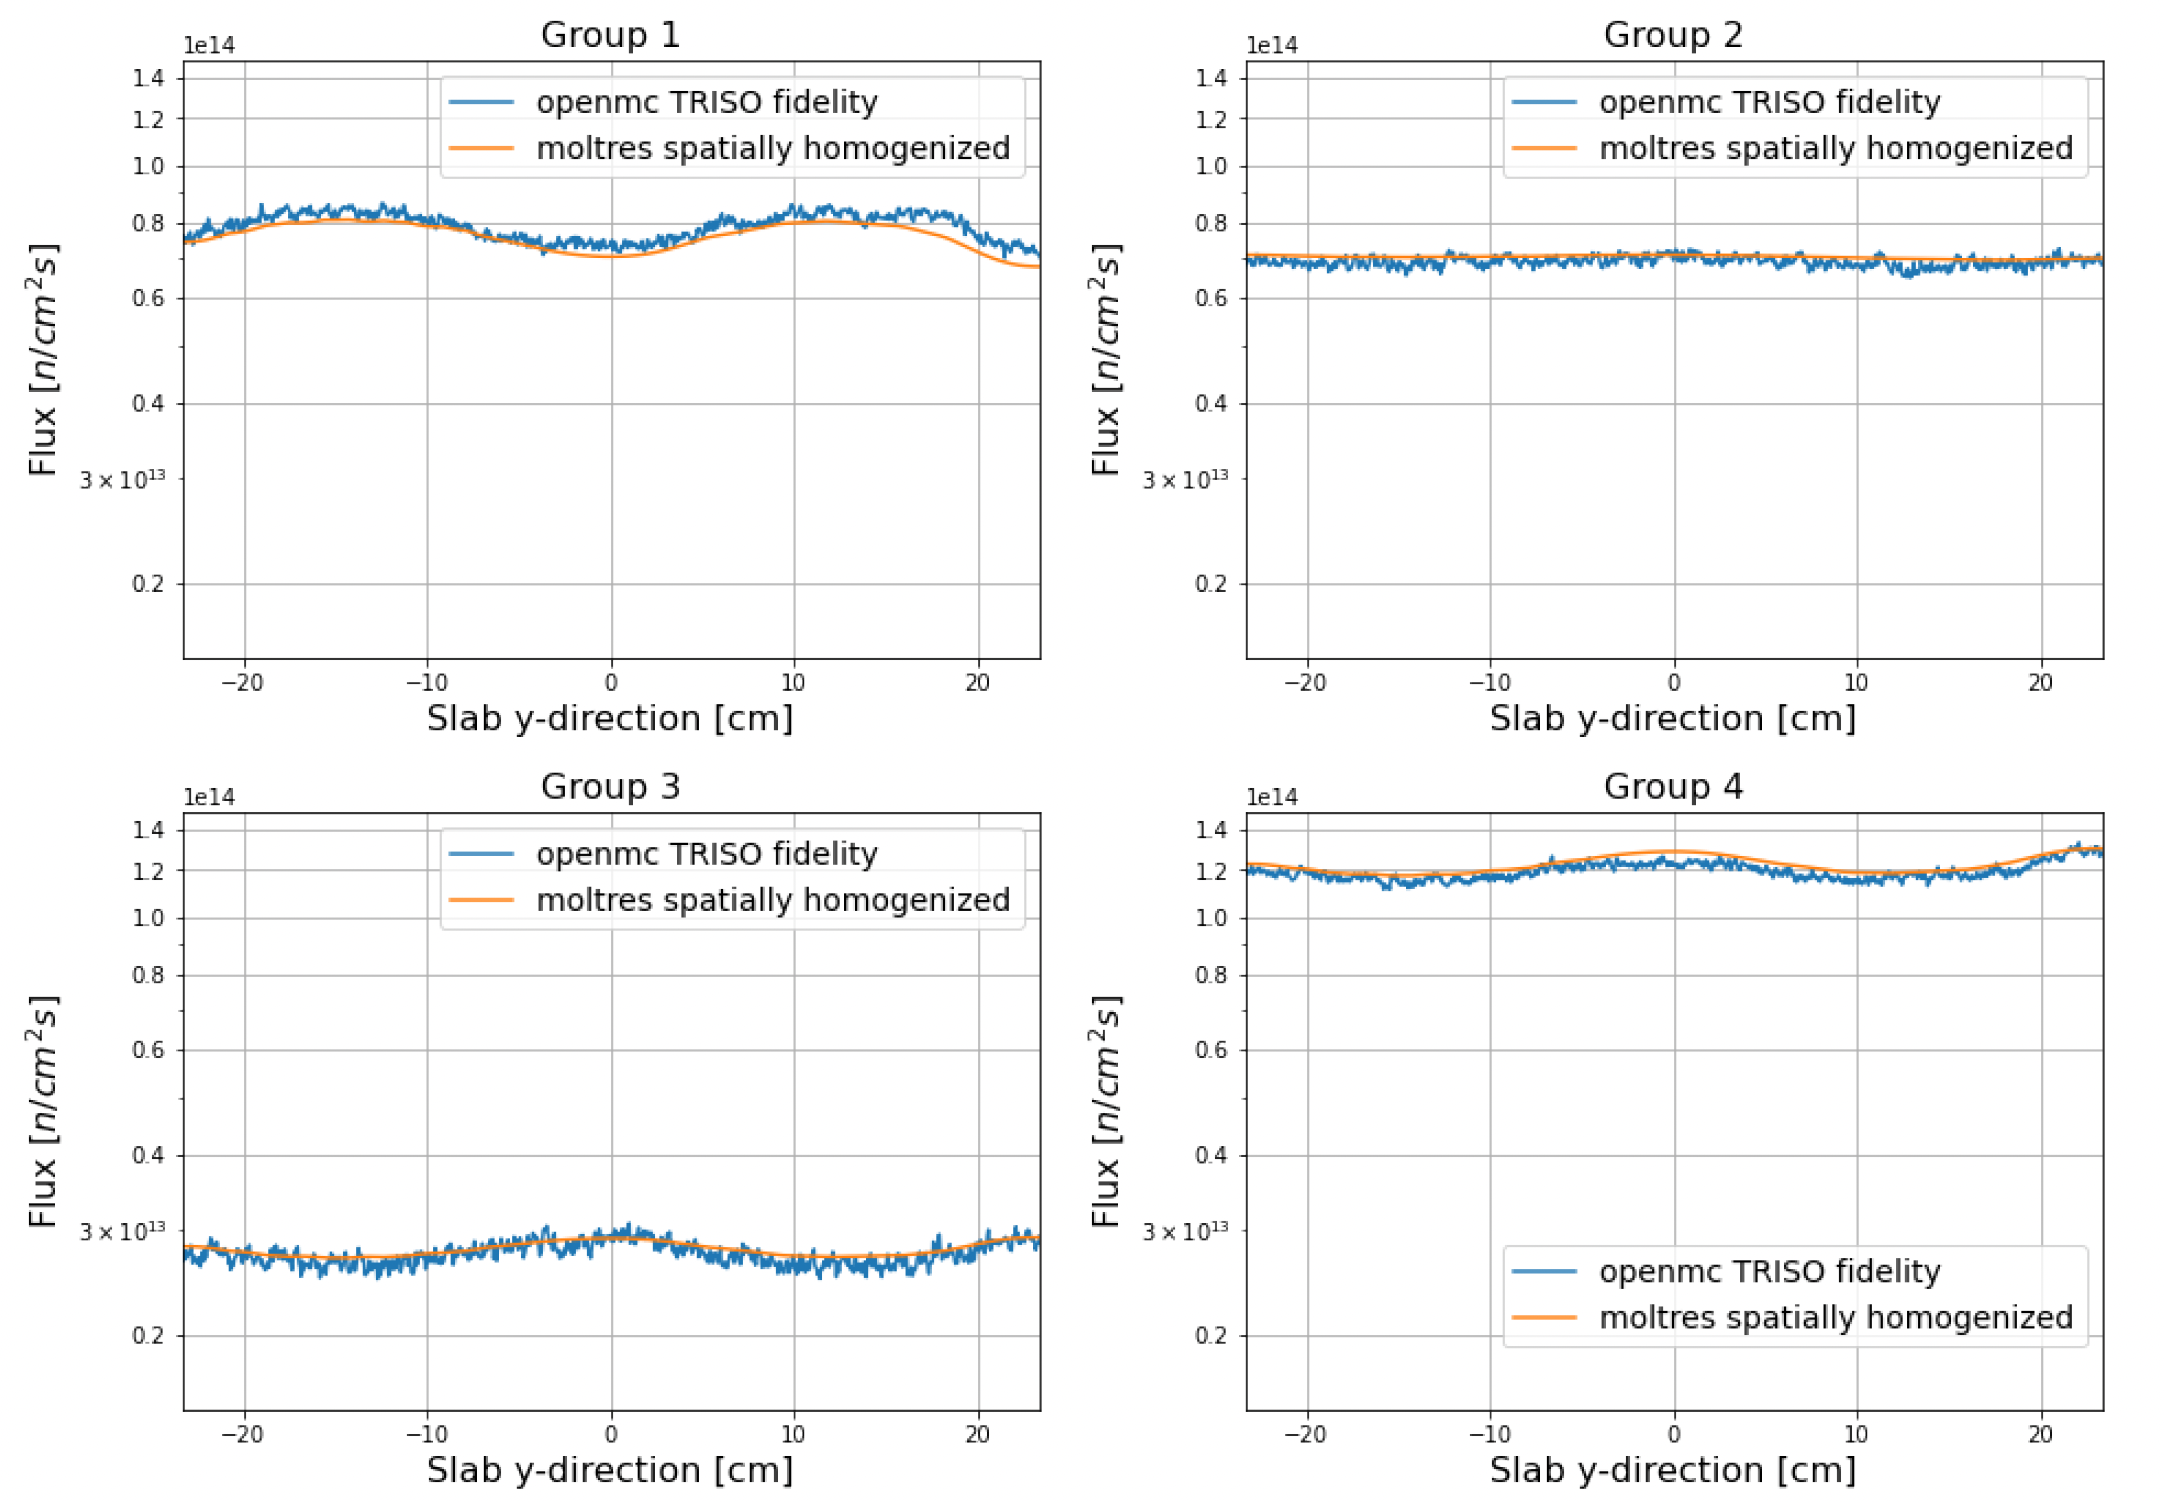
\includegraphics[width=\linewidth]{figures/benchmark-flux.png} 
        \caption{4-group flux distribution comparison.}
    \end{figure}
    \end{column}
    \begin{column}{0.3\textwidth}
        2-norm Diff [\%]
        \begin{itemize}
            \item Group 1: 0.13\% 
            \item Group 2: 0.08\% 
            \item Group 3: 0.10\% 
            \item Group 4: 0.09\%
        \end{itemize}
        Max Diff [\%]
        \begin{itemize}
            \item Group 1: -10.57\% 
            \item Group 2: +7.58\% 
            \item Group 3: +8.96\% 
            \item Group 4: +6.97\%
        \end{itemize}
    \end{column}
    \end{columns}
\end{frame}

\begin{frame}
    \frametitle{AHTR Temp Model Neutron Energy Spectrum Verification}
            \begin{figure}[]
                \centering
                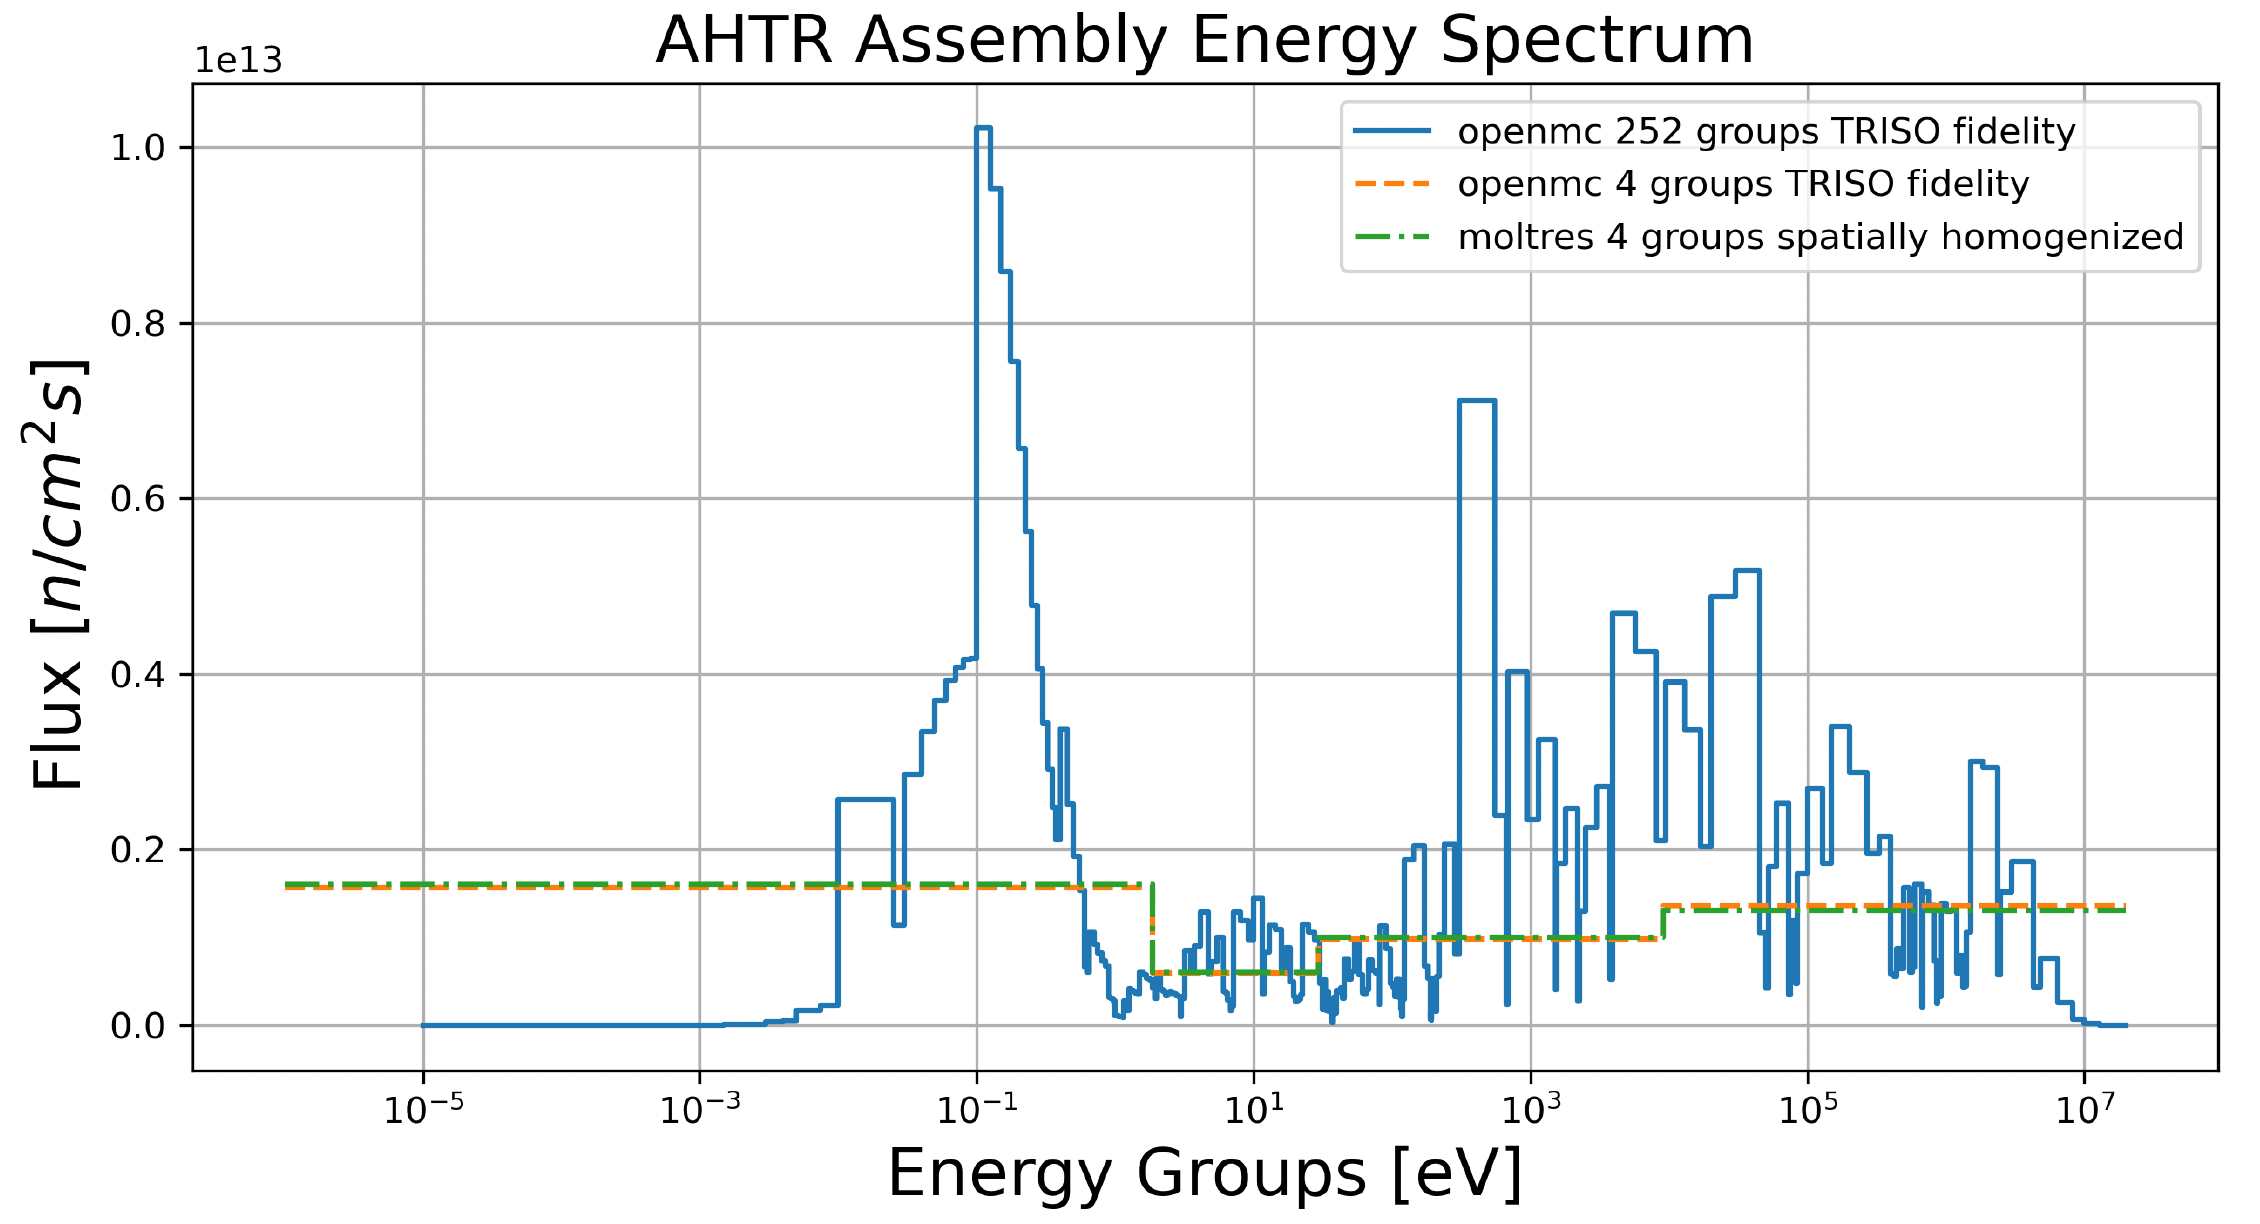
\includegraphics[width=0.75\linewidth]{figures/benchmark-spectrum.png} 
                \caption{Neutron Energy Spectrum Comparison.}
            \end{figure}
        \textbf{Good agreement} between OpenMC and Moltres models 4-group spectrums.
\end{frame}

\subsection{TRISO Particle Homogenization}
\begin{frame}
    \frametitle{TRISO Particle Homogenization}
    \begin{table}
        \caption{Straightened \acrfull{AHTR} fuel plank $k_{eff}$ for the case with 
        no \gls{TRISO} homogenization and case with homogenization of the four outer 
        layers. Both simulations were run on one BlueWaters supercomputer XE Node 
        using OpenMC with 80 active 
        cycles, 20 inactive cycles, and 8000 particles.}
        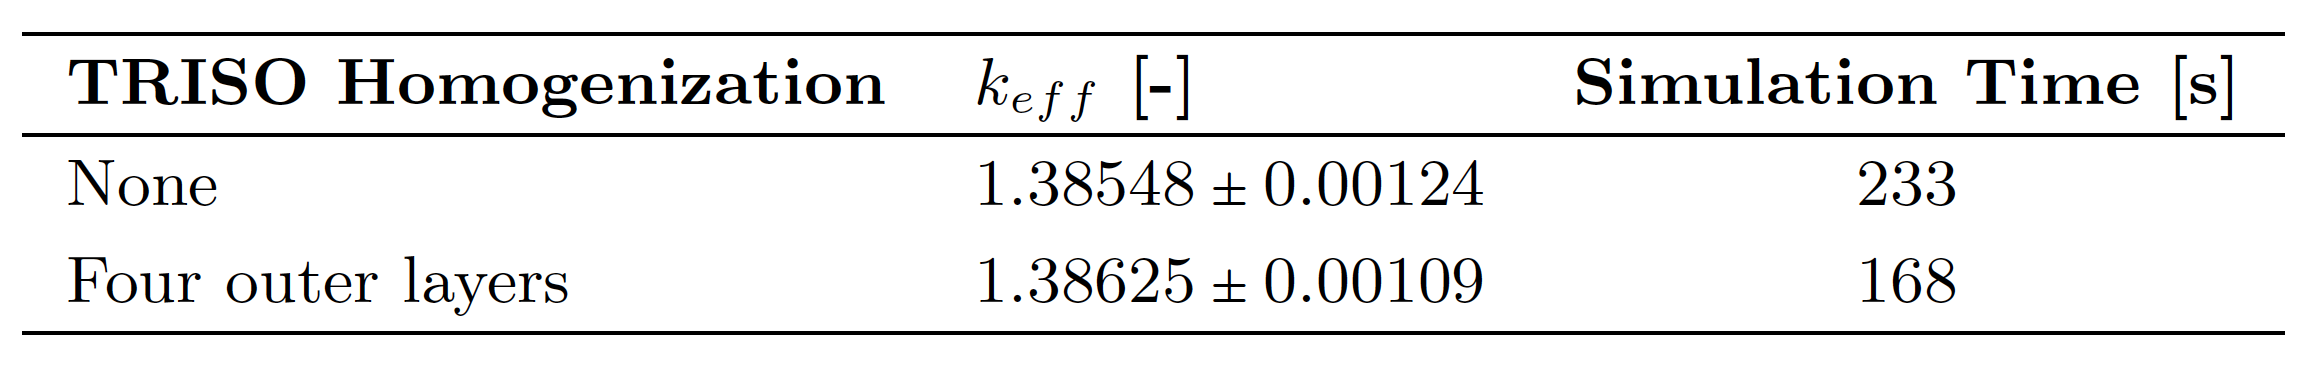
\includegraphics[width=0.75\linewidth]{figures/triso-homogenization.png} 
    \end{table}

    The \gls{TRISO} particle outer four-layer homogenization resulted in a $30\%$ 
    speed-up without compromising accuracy with $k_{eff}$ values within each 
    other's uncertainty.

    As a result, the homogenized models are used for all subsequent optimization efforts. 

\end{frame}

\subsection{ROLLO Verification}
\begin{frame}
    \frametitle{ROLLO Successfully Verified with $^{239}Pu$ Critical Bare Sphere}
    \begin{figure}
        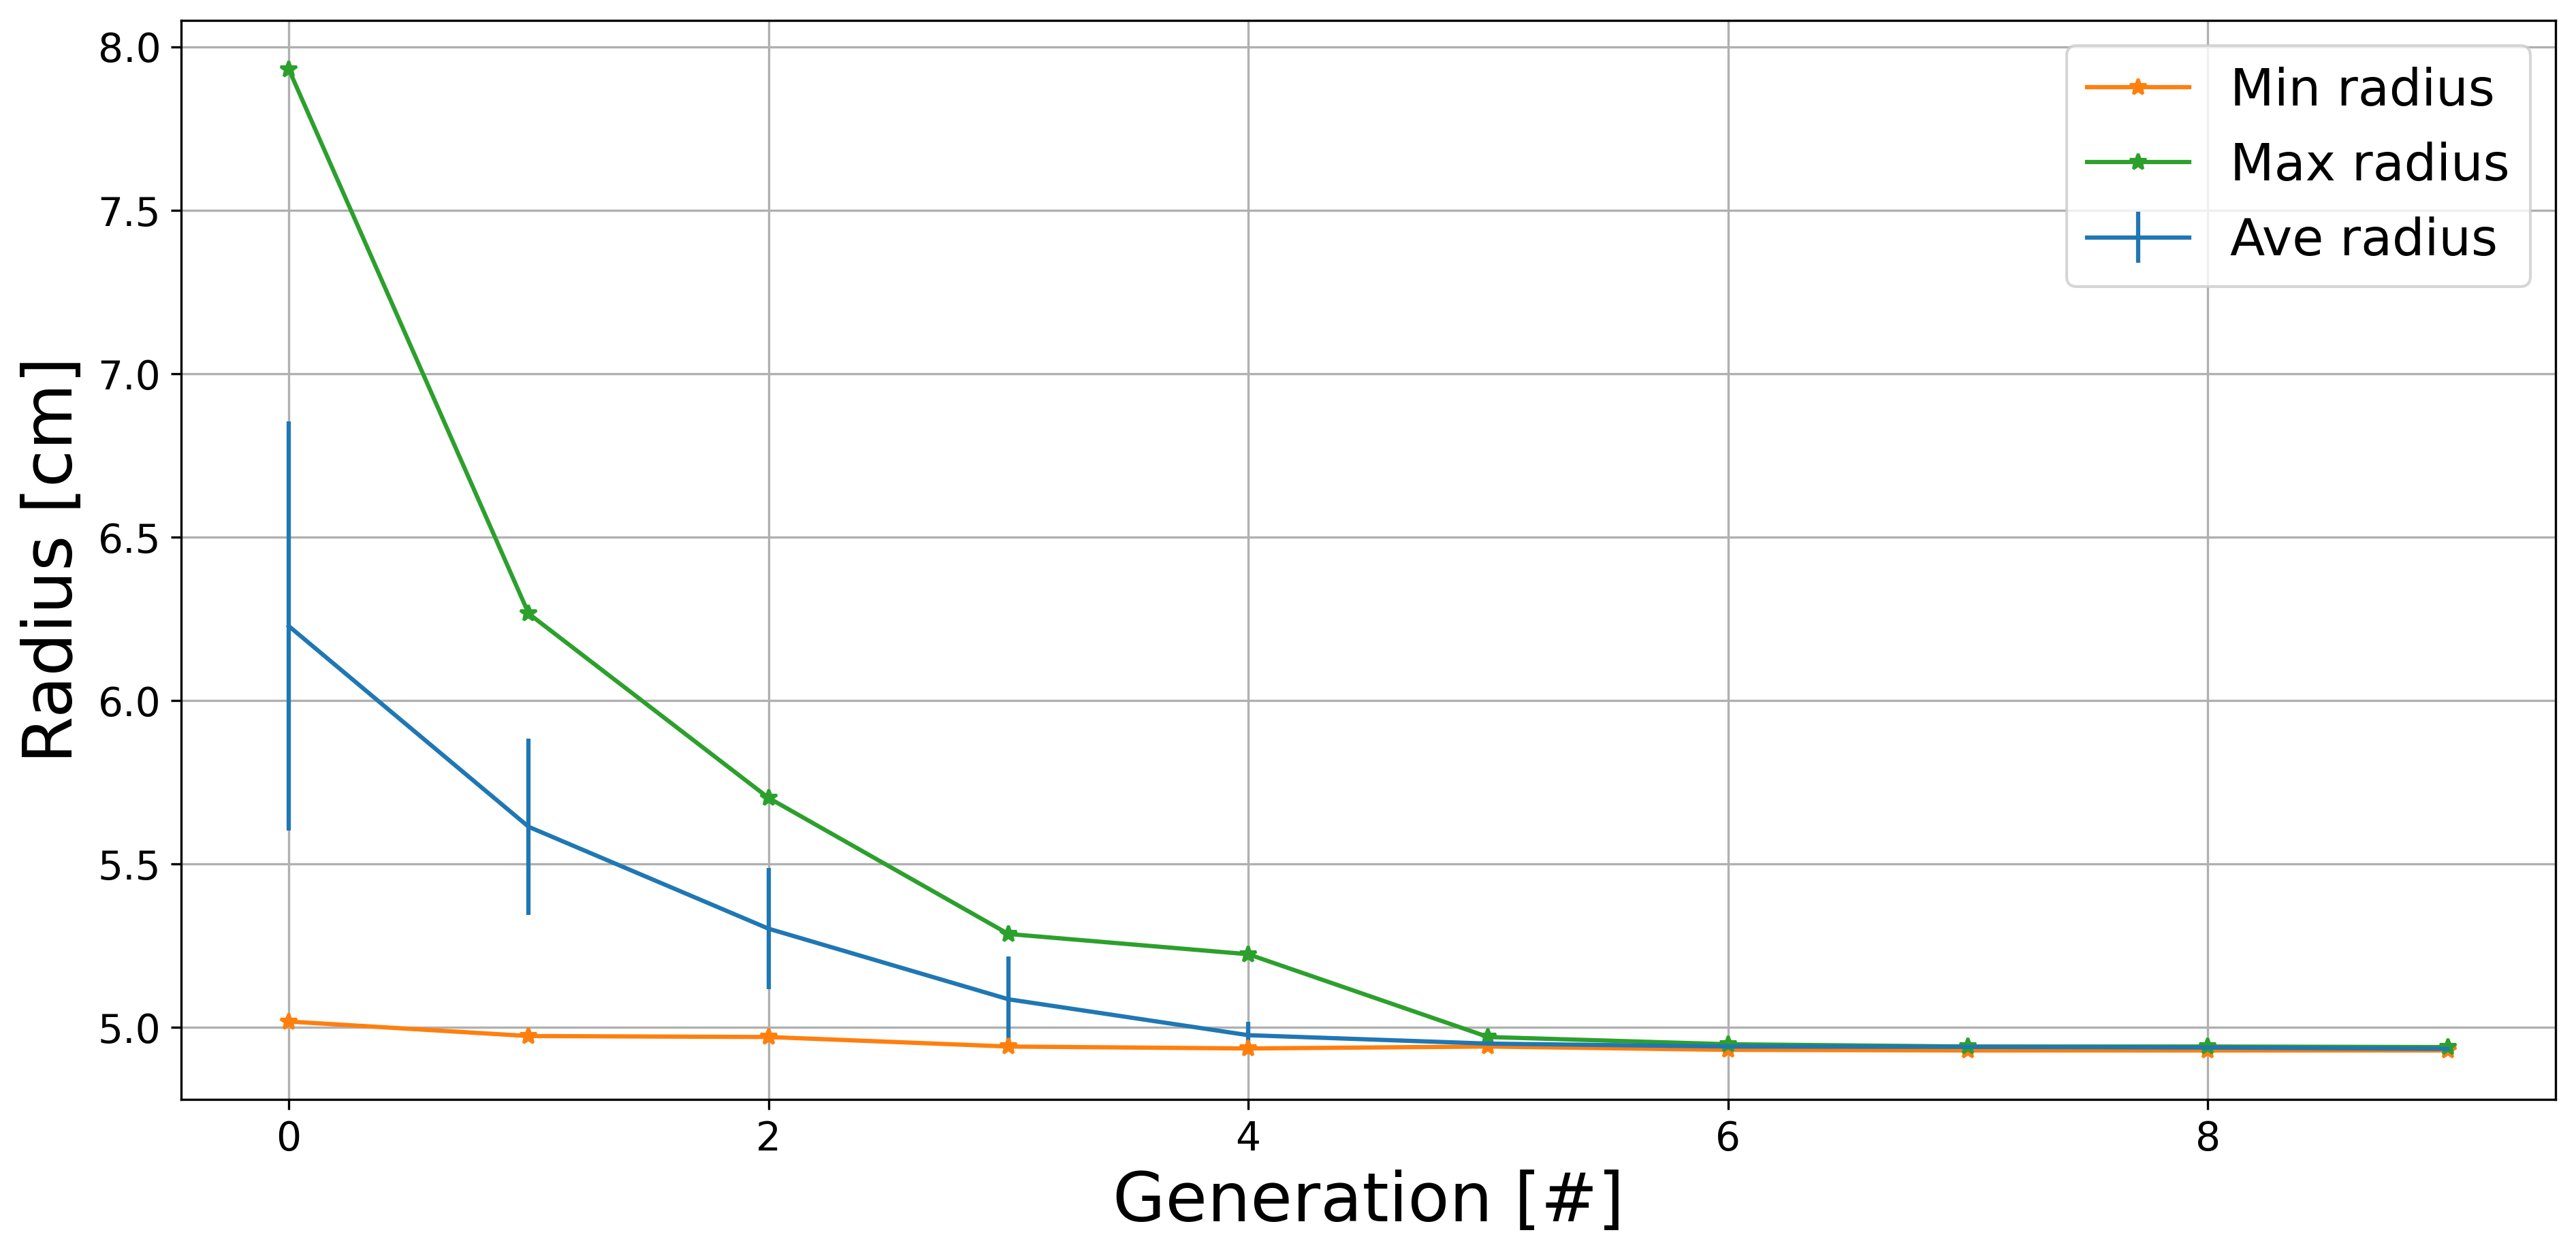
\includegraphics[width=0.85\linewidth]{../docs/figures/radius-convergence.png} 
        \caption{Results for each generation for \gls{ROLLO}'s genetic algorithm 
        optimization to the find the critical radius of a  $^{239}Pu$ bare sphere.}
    \end{figure}
    \vspace{-0.2cm}
    \textbf{ROLLO successfully finds the critical radius of the $^{239}Pu$ bare sphere 
    to be 4.9856cm.}
\end{frame}

\begin{frame}
    \frametitle{ROLLO $^{239}Pu$ Critical Bare Sphere Input File}
    \begin{figure}
        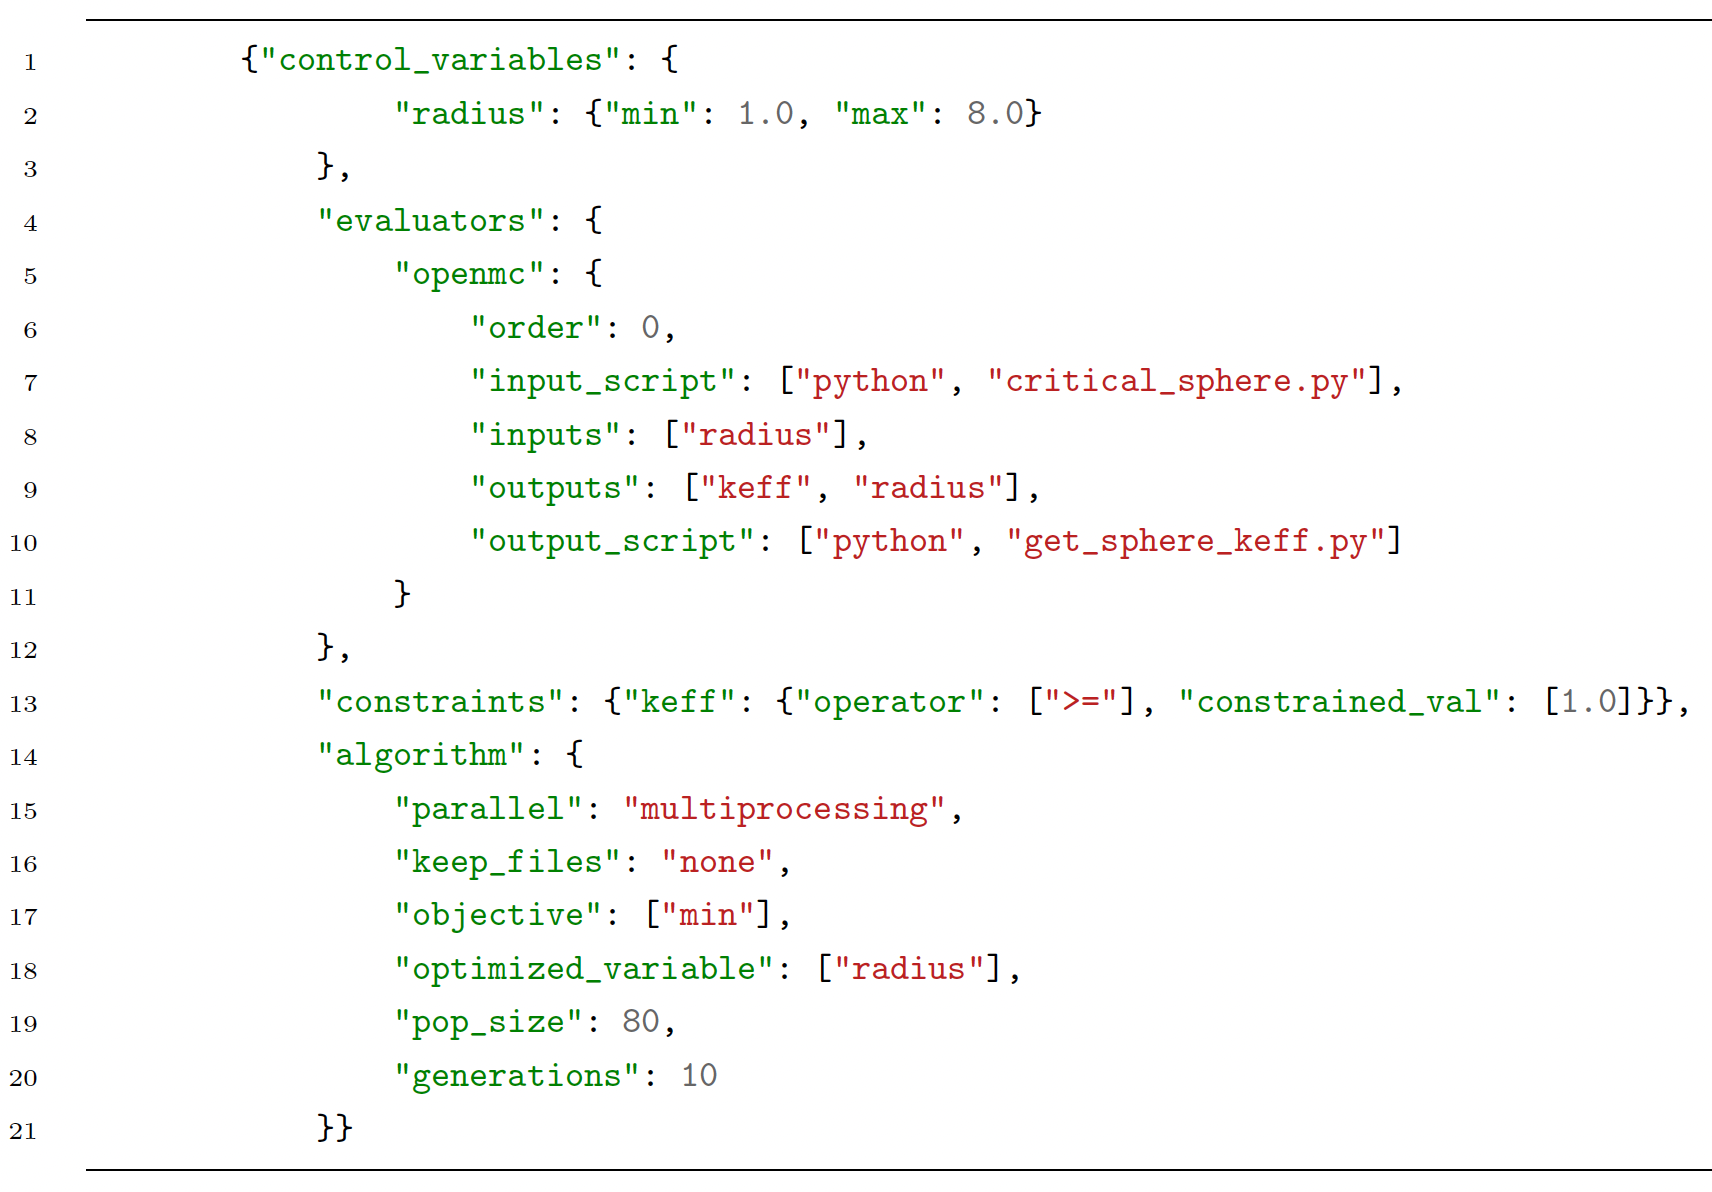
\includegraphics[width=0.49\linewidth]{figures/rollo-verify-file.png} 
        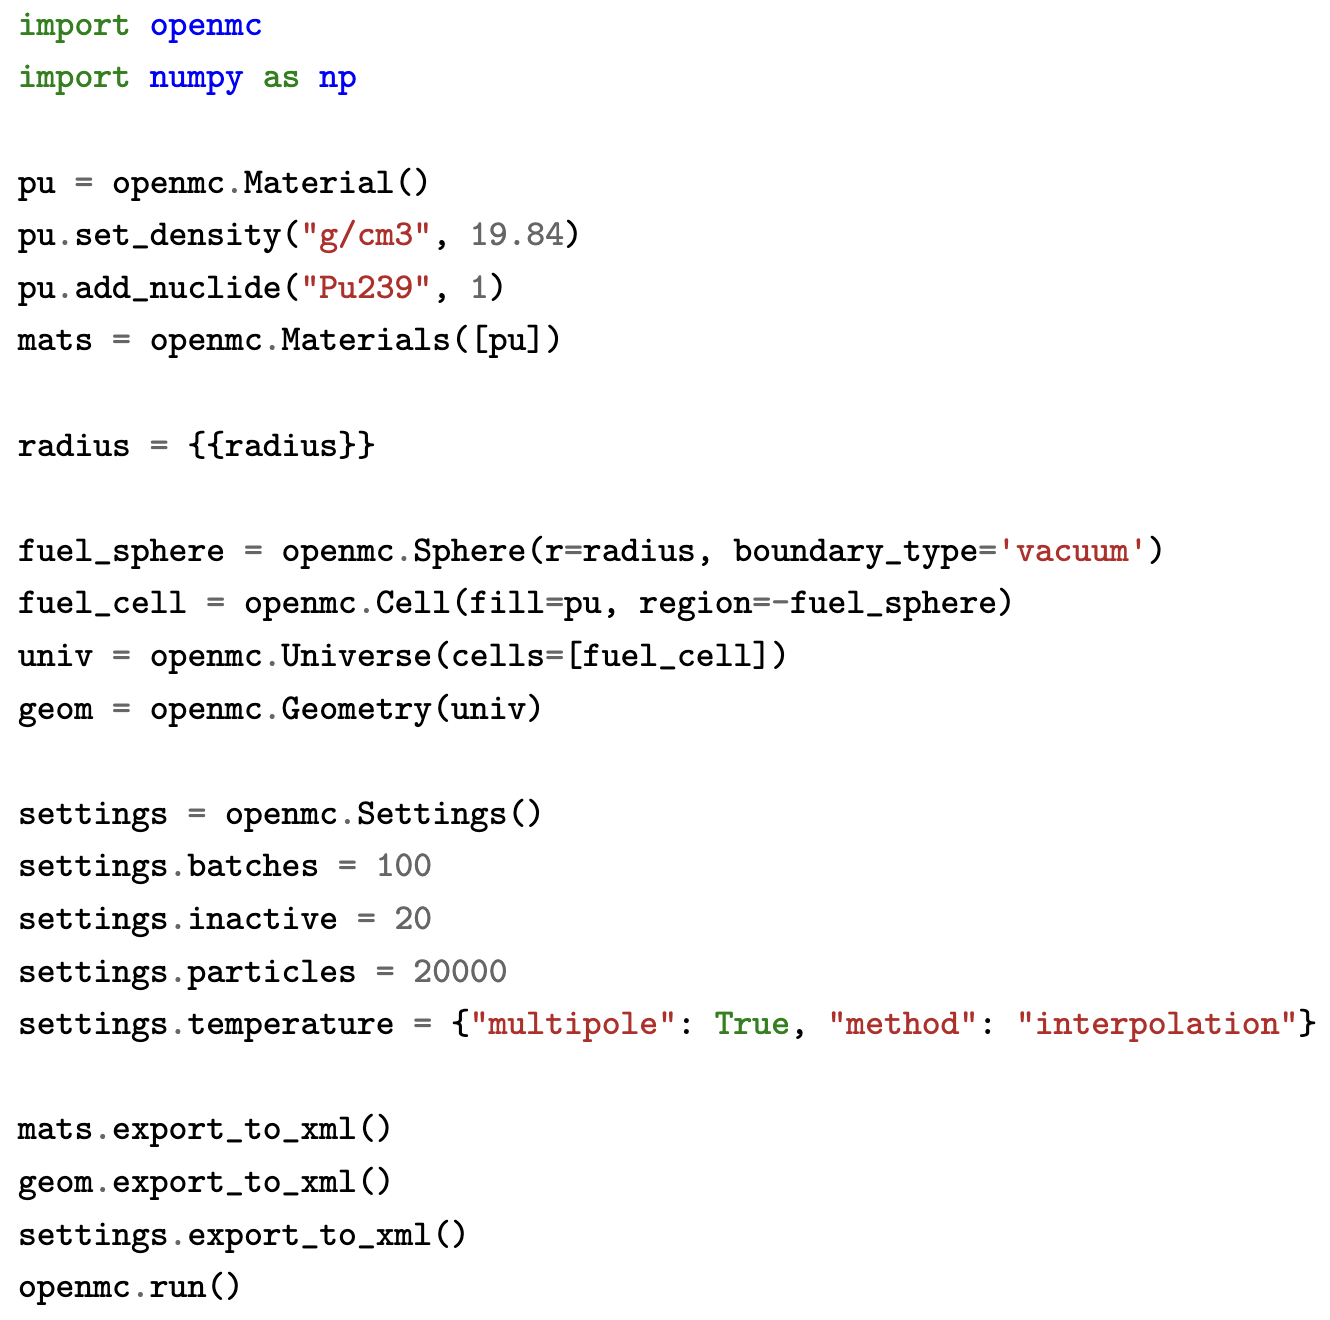
\includegraphics[width=0.49\linewidth]{figures/rollo-verify-file2.png}
        \caption{ROLLO $^{239}Pu$ Critical Bare Sphere Input File.}
    \end{figure}
\end{frame}

\begin{frame}
    \frametitle{AHTR Plank Geometry}
    A sine distribution governs TRISO packing fraction distribution: 
    \begin{align}
        \rho_{TRISO}(\vec{x}) &= \left(\textbf{a}\cdot sin(\textbf{b}\cdot x + \textbf{c}) + 2\right) \cdot NF \nonumber
    \end{align}
    \begin{figure}
        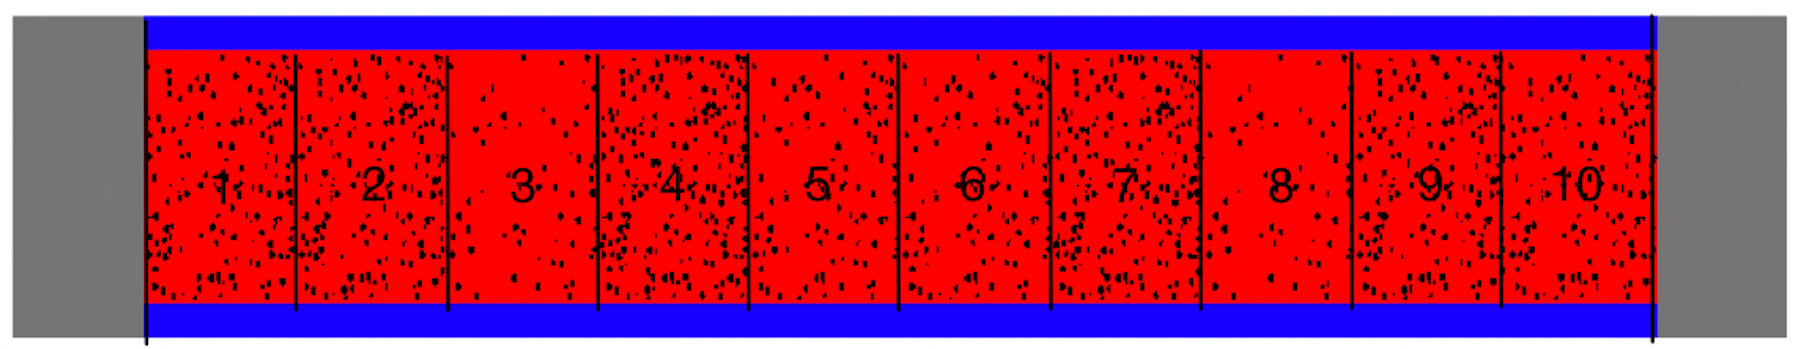
\includegraphics[width=0.9\linewidth]{../docs/figures/straightened_plank.png} 
        \caption{Straightened AHTR Plank with 10 fuel cells with random TRISO packing.}
    \end{figure}
    $r_{top}$ and $r_{bot}$ control coolant channel shape: 
    \begin{figure}
        
\includegraphics[width=\linewidth]{../docs/figures/coolant-channel-shape.png} 
        \caption{AHTR Plank with coolant channel shape variation, $r_{top}$ = 0.2cm and 
        $r_{bot}$ = 0.3cm.}
    \end{figure}
\end{frame}

\begin{frame}
    \frametitle{Simulation a-3b hypervolume}
    \begin{table}
        \caption{Simulation a-3b hypervolume values at each generation.}
        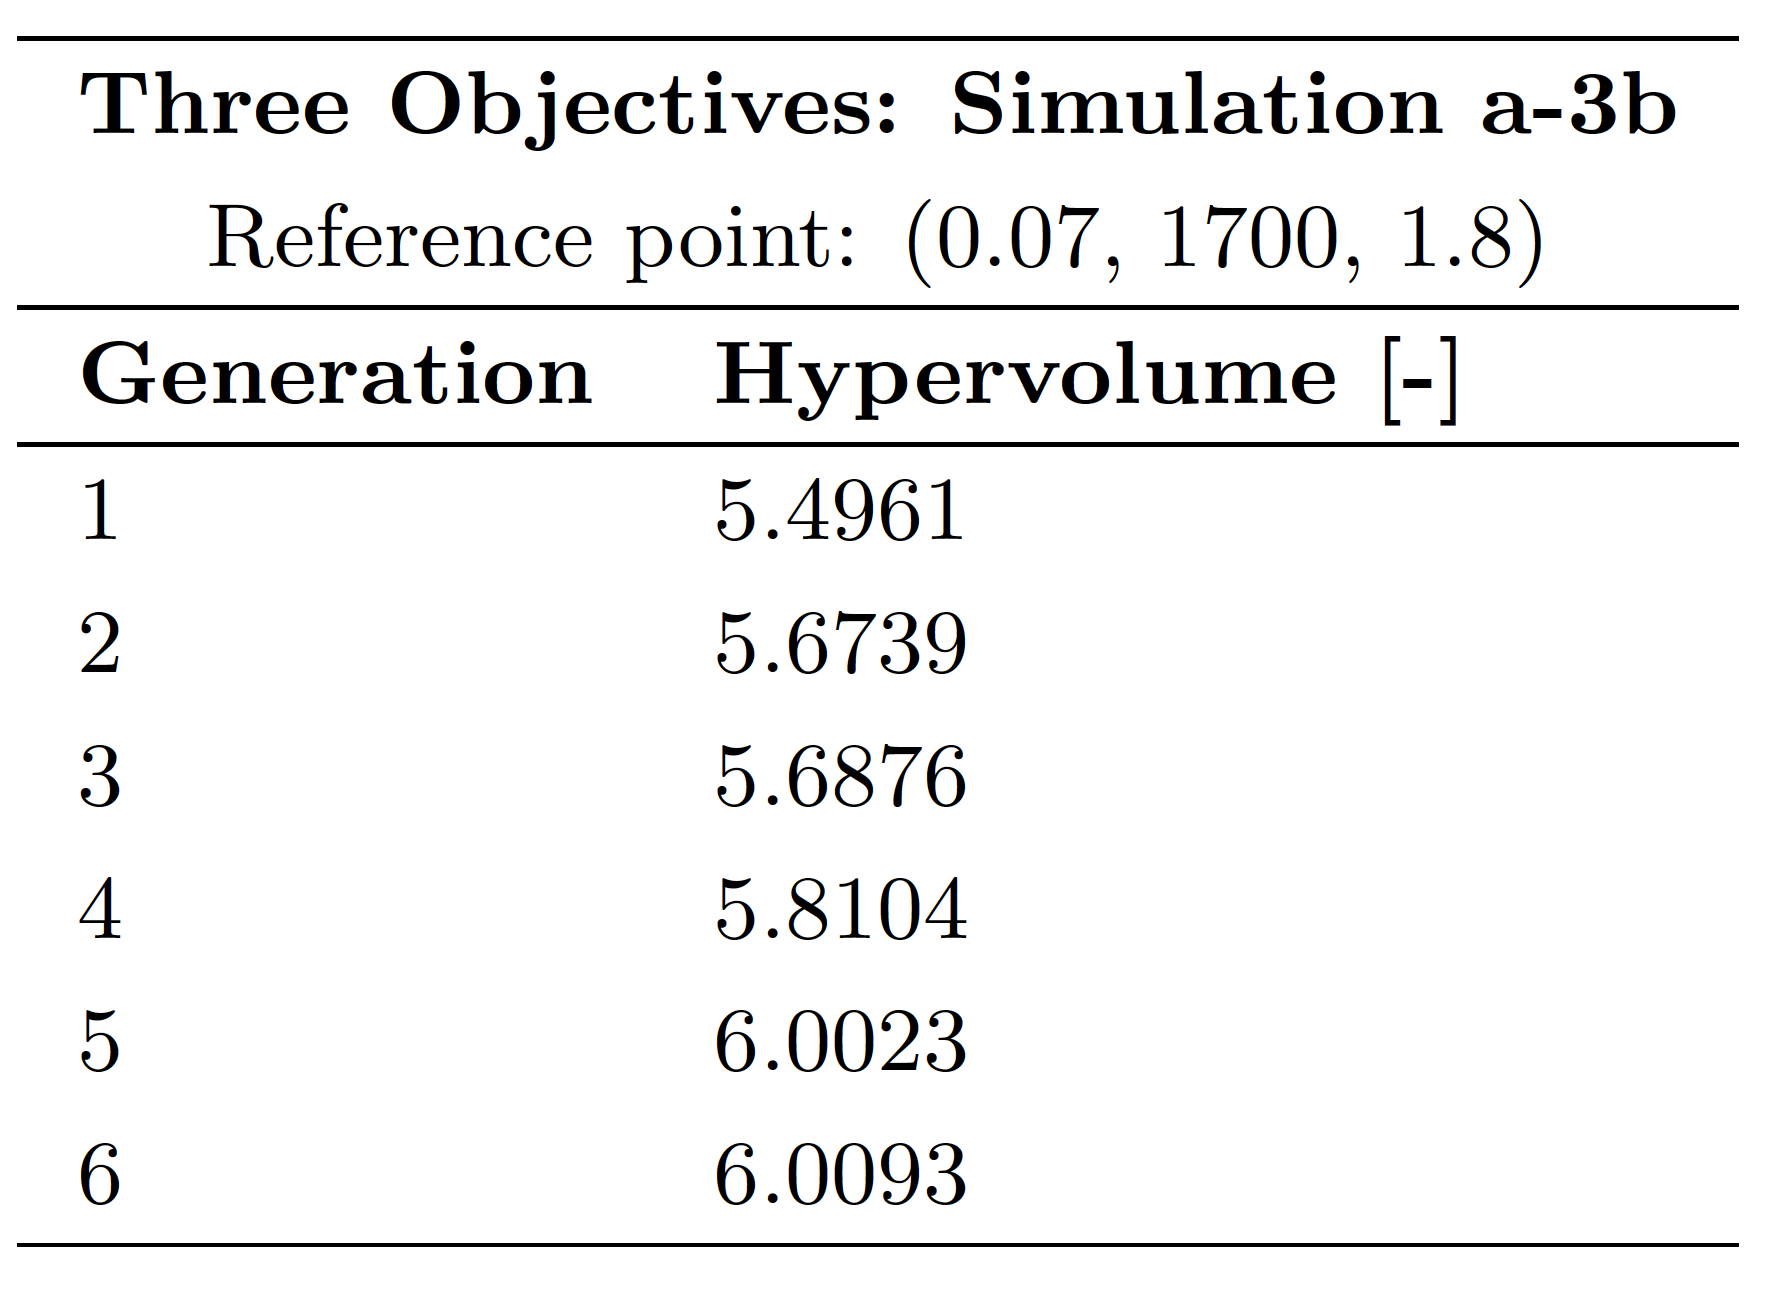
\includegraphics[width=0.4\linewidth]{figures/a-3b-hypervolume.png} 
    \end{table}

    For each optimization simulation, I must balance convergence and computational cost.

    The hypervolume is calculated by finding the volume between the reference point and 
    the objective values of the Pareto front's reactor models (bigger hypervolume = 
    more converged solution).

    I determine if convergence criteria is met by evaluating if the difference between 
    generations' hypervolume values are getting smaller.
\end{frame}

%%--------------------------------%%


\end{document}



